\documentclass[prd,aps,twocolumn,a4paper,showkeys,nofootinbib]{revtex4-1}

\usepackage{amsmath}
\usepackage{amsfonts}
\usepackage{amssymb}	
\usepackage{graphicx}
\usepackage{color}
\usepackage[hidelinks]{hyperref}
\allowdisplaybreaks

\def\TODO{\textcolor{red}{TODO:}}
\def\Mc{{\cal M}_c}

\begin{document}

\title{Regression with Dense Neural Network using TensorFlow}

\author{Simone Albanesi, Marina Berbel}

\date{\today}

\maketitle

%==========================================================
\section{Introduction}
%==========================================================
Working notes on the regression part with a dense Neural Network (NN)
using \texttt{Keras} with \texttt{TensorFlow} in back-end. We use this framework since allows us to
exploit the flexibility of NNs (while \texttt{Scikit-learn} doesn't).

The task is to apply the NN to the quantities recovered from \texttt{GstLAL} $x$ and to predict
values $y^{\rm pred} = f\left( x \right)$ that are a better approximation of the injected 
values $y^{\rm true}$.

Some pros of NNs are:
\begin{itemize}
\item virtually infinite number of architectures, many aspects to tune on our problem 
\item they are used everywhere nowadays, so it is easy to find material online
\item is possible to put constraints on the output
\item easy to customize
\end{itemize}
On the other hand, to fully exploit the NN we need a big dataset and the high number of tunable
aspects makes the cross validation more difficult. In our case we will use at most 2 hidden layers.
In principle more complex architectures could  be used but in our case 
I don't think it would be worth since we do not have a huge training sample. 
For regression tasks, the activation function in the output layer generally is a linear function.

Steps of the regression:
\begin{enumerate}
\item \textbf{Normalization of the data}. The usual normalization (\texttt{StandardScaler})
trasforms the data so that we have zero mean and standard deviation equal to 1. 
Nonetheless I prefer to use the 
linear map \texttt{MinMaxScaler} that maps the data in the interval $[-1,1]$. 
This choice is linked to the constraints on the output, see Sec.~\ref{sec:constraints}. 

\item \textbf{Initialization of the model}. We decide the architecture and all the other aspects. 
A typical configuration is:
\begin{itemize}
\item layers: two layers with 100 neurons, but e.g. on the \texttt{v0c0}
dataset a more complex architecture could be slightly better 
(see Sec.~\ref{sec:crossval} for more info on this);
\item activation function in hidden layers: \texttt{ReLU}. Other options like the sigmoid 
or the hyperbolic tangent require longer training and provide worse results.;
\item activation function in output layer: \texttt{linear};
\item optimizer: \texttt{Adam} (optimized version of the stochastic gradient descent);
\item loss function: \texttt{MeanSquaredError()} (see Sec.~\ref{sec:loss} for more details 
and other options);
\item learning rate: 0.001;
\item epochs and batch-size: a good combination is 250 and 32, respectively. Sometimes I use a
bigger batch-size to speed-up the training (e.g. I used 128 for the cross-validation on
the \texttt{v0c0} dataset).
\end{itemize}

\item \textbf{Training}. Using  the dataset \texttt{v0c0}, $N_{\rm epochs}=250$ and 
$N_{\rm batch}=128$ the training
takes from 60 to 90 seconds, depending on the architecture. During the training we also 
use the $20\%$ of the training dataset for the validation so that
we can monitor the loss and the $R^2$ coefficient (see definition below) at each epoch.

\item \textbf{Evaluation of the accuracy}. To evaluate the goodness of the model 
we use the coefficient of determination $R^2=1-SS_{\rm res}/SS_{\rm tot}$, where
$SS_{\rm res}=\sum{(y^{\rm true}_i-f(x_i))^2}$, 
$SS_{\rm tot}=\sum{(y^{\rm true}_i - \bar{y}^{\rm true})^2}$, 
and $\bar{y}^{\rm true}$ is the mean. This is also the \texttt{score} 
of \texttt{Scikit-learn}. It is better to evaluate the $R^2$ coefficient
for each feature instead of a global $R^2$. 
\end{enumerate}

%==========================================================
\section{Constraints on the output}
%==========================================================
\label{sec:constraints}
We need some constraints on the output since we don't want to predict negative masses 
or naked singularities. A solution is to modify the activation function 
$\sigma$ in the output layer.
Another option could be to enforce the constraints in the loss function, but I have not tried this
(and in any case this would not guarantee physical predictions). 
The idea is to make $\sigma$ saturate when the prediction is out of the physical range. 
The first step is to normalize the data in the interval $[-1,1]$ using the \texttt{MinMaxScaler}.
Then for $\sigma$ we use the following prescription:
\begin{equation}
\hat{\sigma}(x) = \begin{cases} 
      -1 & x\leq -1 \\
      x & -1\leq x\leq 1 \\
      1 & x \geq 1 
\end{cases}
\end{equation}
Using a sigmoid ansatz is possible to find a smooth approximants
\begin{equation}
\sigma^N(x)  = \frac{2}{e^{-2 f^N(x)}+1}-1,
\end{equation}
where 
\begin{equation}
f^N(x)  = \sum_{n=odd}^{N} \frac{x^{n}}{n}.
\end{equation}
The function $f^N(x)$ is  simply found requiring that $\sigma^N(x)=x+O(x^{N+2})$ 
for $x\rightarrow 0$.
These activation functions are shown in the left panel of Fig.~\ref{fig:out_act_f}.
%
\begin{figure}[t]
  \center
  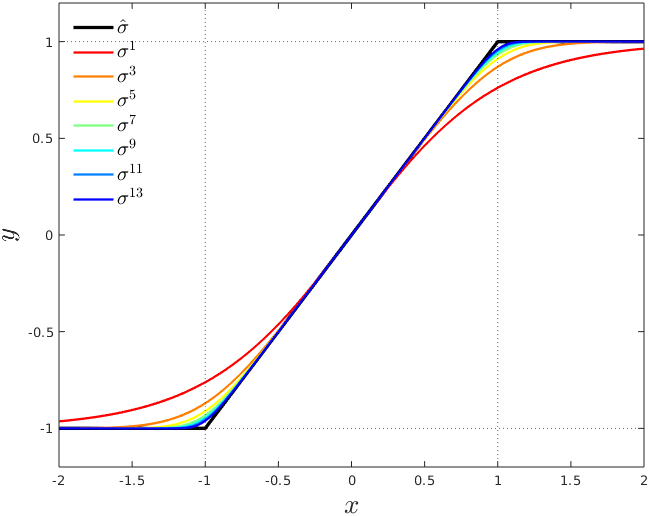
\includegraphics[width=0.23\textwidth,height=3.7cm]{./Figs/out_activation_function.png}
  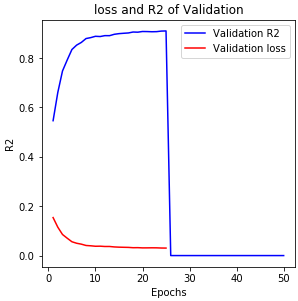
\includegraphics[width=0.23\textwidth,height=3.9cm]{./Figs/history_sigma5_layers20+20.png}
  \caption{\label{fig:out_act_f} \textbf{Left panel}: activation functions to use in the 
  output layer so that the output is constrained in the interval $[-1,1]$.
  \textbf{Right panel}: history of a NN with two hidden layers with 20 neurons 
  and $\sigma^5(x)$ as output function.
  The drop in the accuracy at the 18th epoch is due to the presence of NaN.
  That's why we use $\hat{\sigma}$ and not a smooth approximant $\sigma^N$.}
\end{figure}
%
However, for $N\geq 3$ is possible that some NaN appear during the training, see e.g. the right
panel of Fig.~\ref{fig:out_act_f} where we show a case with $\sigma^5(x)$. 
I remember that once also $\sigma^3(x)$ failed, but I 
cannot find this configuration again (is a rare event). 
In any case to be safe I will use the piecewise function $\hat{\sigma}$ ($\sigma^1(x)$ is 
not steep enough).
Clearly it is also possible to saturate only the upper of the lower boundary, in particular we 
for the masses I will often use
\begin{equation}
\hat{\sigma}_{\rm LB}(x) = \begin{cases} 
      -1 & x\leq -1 \\
      x & -1\leq x.
\end{cases}
\end{equation}
However I am not sure that removing the upper boundary makes sense, maybe it would 
be better to use the upper constraint also for the masses, TBD.
%
\begin{table}[t]
\caption{\label{tab:some_results} Loss (Mean Squared Error) and $R^2$ coefficients
 	for the two datasets \texttt{v0c0}, \texttt{v1c0}.
   	We used 2 hidden layers with 100 neurons, $N_{\rm batch}=64$, 250 epochs,  
   	constrained output. See Sec.~\ref{sec:some_results} for discussion.}
\begin{center}
%\begin{ruledtabular}
\begin{tabular}{c | c | c} 
 & \texttt{v0c0} & \texttt{v1c0}  \\
\hline
\hline
loss (MSE)      & 0.0079 & 0.0533 \\
\hline
$R^2$ mean      & 0.9652 & 0.7533 \\
\hline
$R^2 [m_1   ]$  & 0.9962 & 0.8938 \\
$R^2 [m_2   ]$  & 0.9860 & 0.9454 \\
$R^2 [s^1_x ]$  & 0.9582 & 0.6134 \\
$R^2 [s^1_y ]$  & 0.9529 & 0.6344 \\
$R^2 [s^1_z ]$  & 0.9549 & 0.6436 \\
$R^2 [s^2_x ]$  & 0.9539 & 0.6853 \\
$R^2 [s^2_y ]$  & 0.9570 & 0.6409 \\
$R^2 [s^2_z ]$  & 0.9568 & 0.6468 \\
$R^2 [\theta]$  & 0.9073 & 0.6648 \\
$R^2 [q     ]$  & 0.9957 & 0.9244 \\
$R^2 [M_c   ]$  & 0.9978 & 0.9938 
\end{tabular}
%\end{ruledtabular}
\end{center}
\end{table}

%==========================================================
\section{fake-fake data}
%==========================================================
Section dedicated to the fake-fake data. Things work
properly on these datasets.

%==========================================================
\subsection{Some results}
%==========================================================
\label{sec:some_results}
%
\begin{figure}[]
  \center
  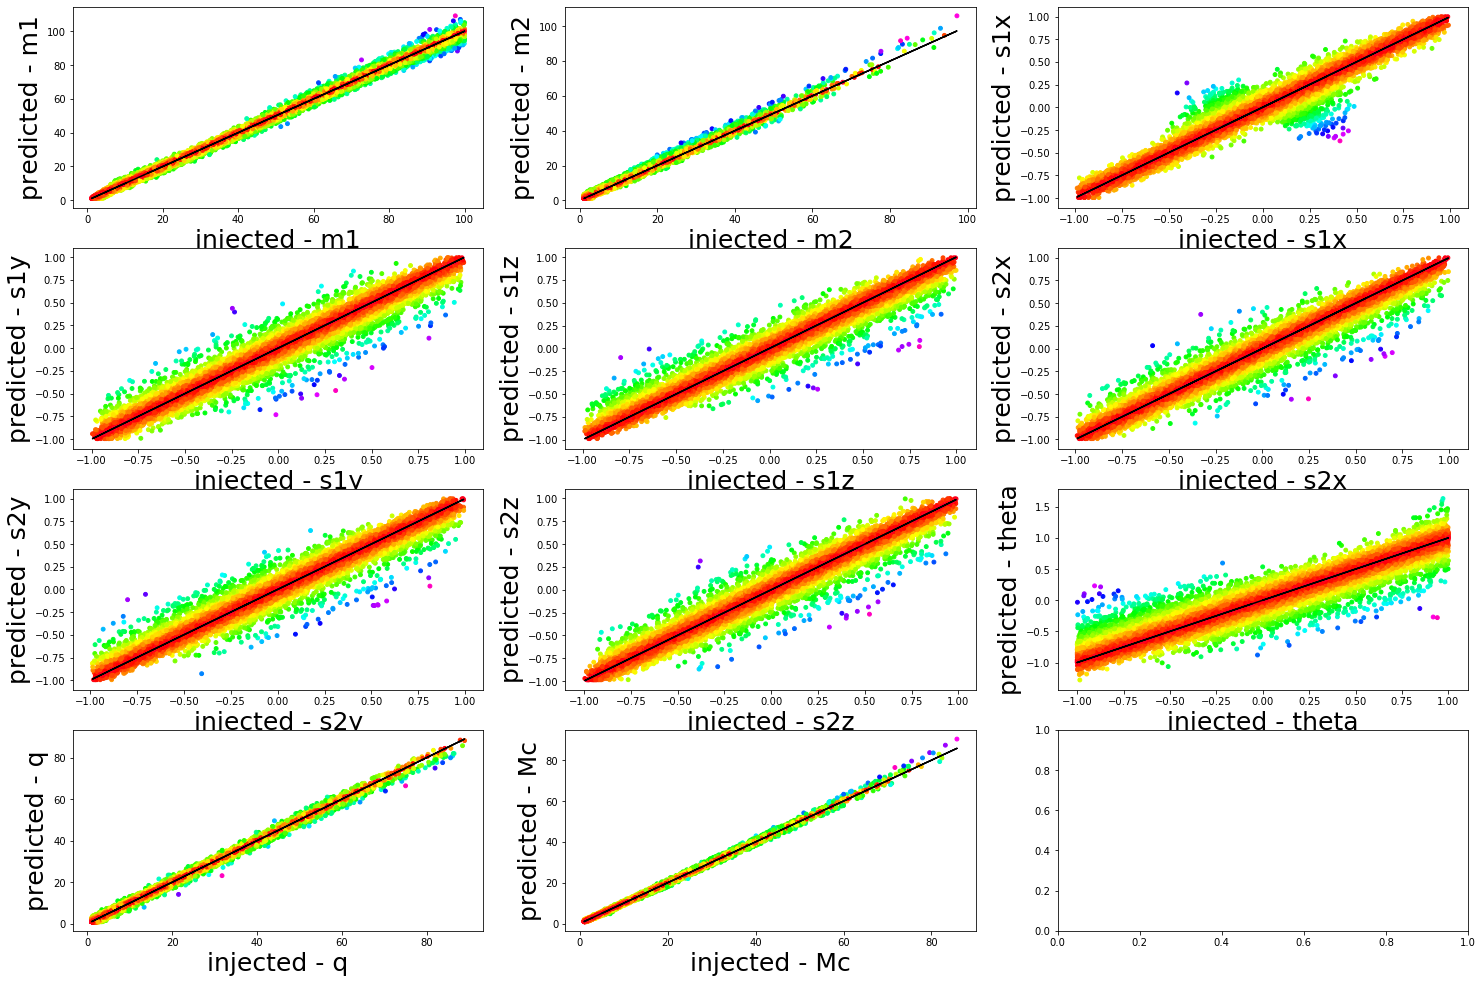
\includegraphics[width=0.45\textwidth]{./Figs/v0c0_regression.png}\\
  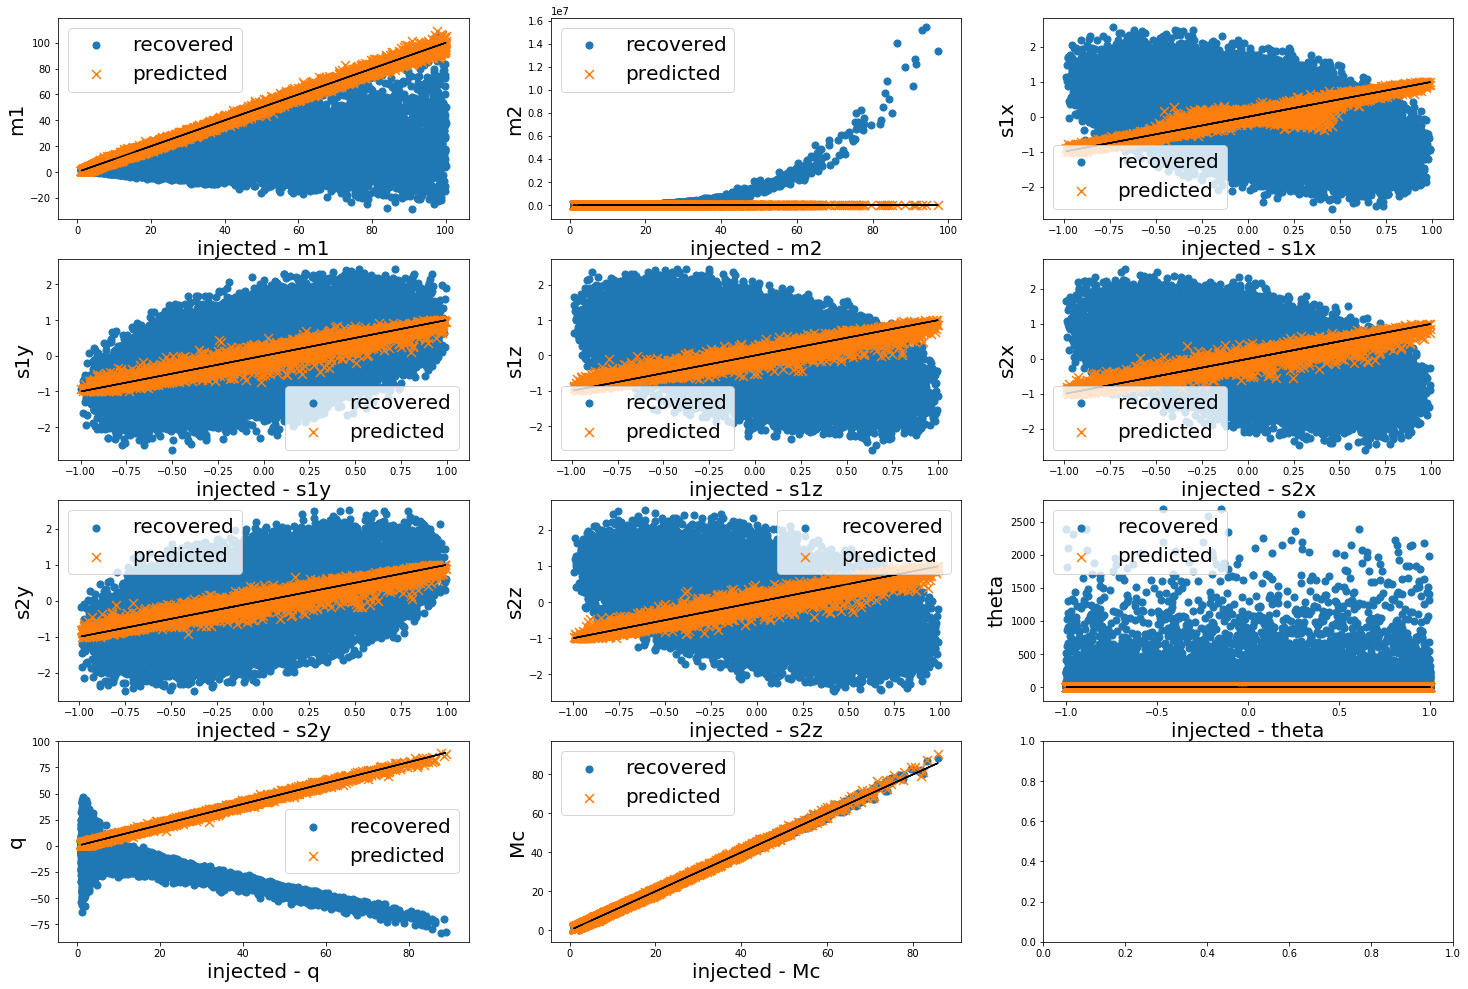
\includegraphics[width=0.45\textwidth]{./Figs/v0c0_regression_noise.png}
  \caption{\label{fig:v0c0_results} Results of the regression on the \texttt{v0c0}
  dataset. We used 2 hidden layers with 100 neurons, $N_{\rm batch}=64$, 250 epochs,  
  constrained output. See Sec.~\ref{sec:some_results} for discussion. 
  The colors in the first plots is related to the absolute difference between predicted 
  and injected. The black line is the bisector.}
\end{figure}
%
The regression with NN works pretty well on the \texttt{v0} datasets, while on 
the dataset \texttt{v1} the $R^2$ coefficients are smaller since there is more degeneracy.
We use 2 hidden layers with 100 neurons (i.e. 12,411 trainable parameters, while
$N_{\rm sample}=2\cdot 10^4$) and we train on 250 epochs using 
$N_{\rm batch}=64$. Different architectures are discussed in Sec.~\ref{sec:crossval}
but the results are more or less the same for complex-enough NNs.
For the spin components we use $\hat{\sigma}$ as output 
activation function, for the masses and the mass ratio we use $\hat{\sigma}_{\rm LB}$ and
a linear function for the angle. 
In Fig.~\ref{fig:v0c0_results}, Fig.~\ref{fig:v1c0_results} and Table~\ref{tab:some_results}
there are the results for this model.
In the first plots we plot the predicted value against the injected values, while in the seconds
we plot the prediction (orange) on the recovered (blue). Note that the recovered here are not 
physically consistent but it is ok since the main goal at this point 
is to see if a neural network is able to 
recover the original quantities. The relevant thing is that we are able to predict values
that have physical meaning.
%
\begin{figure}[]
  \center
  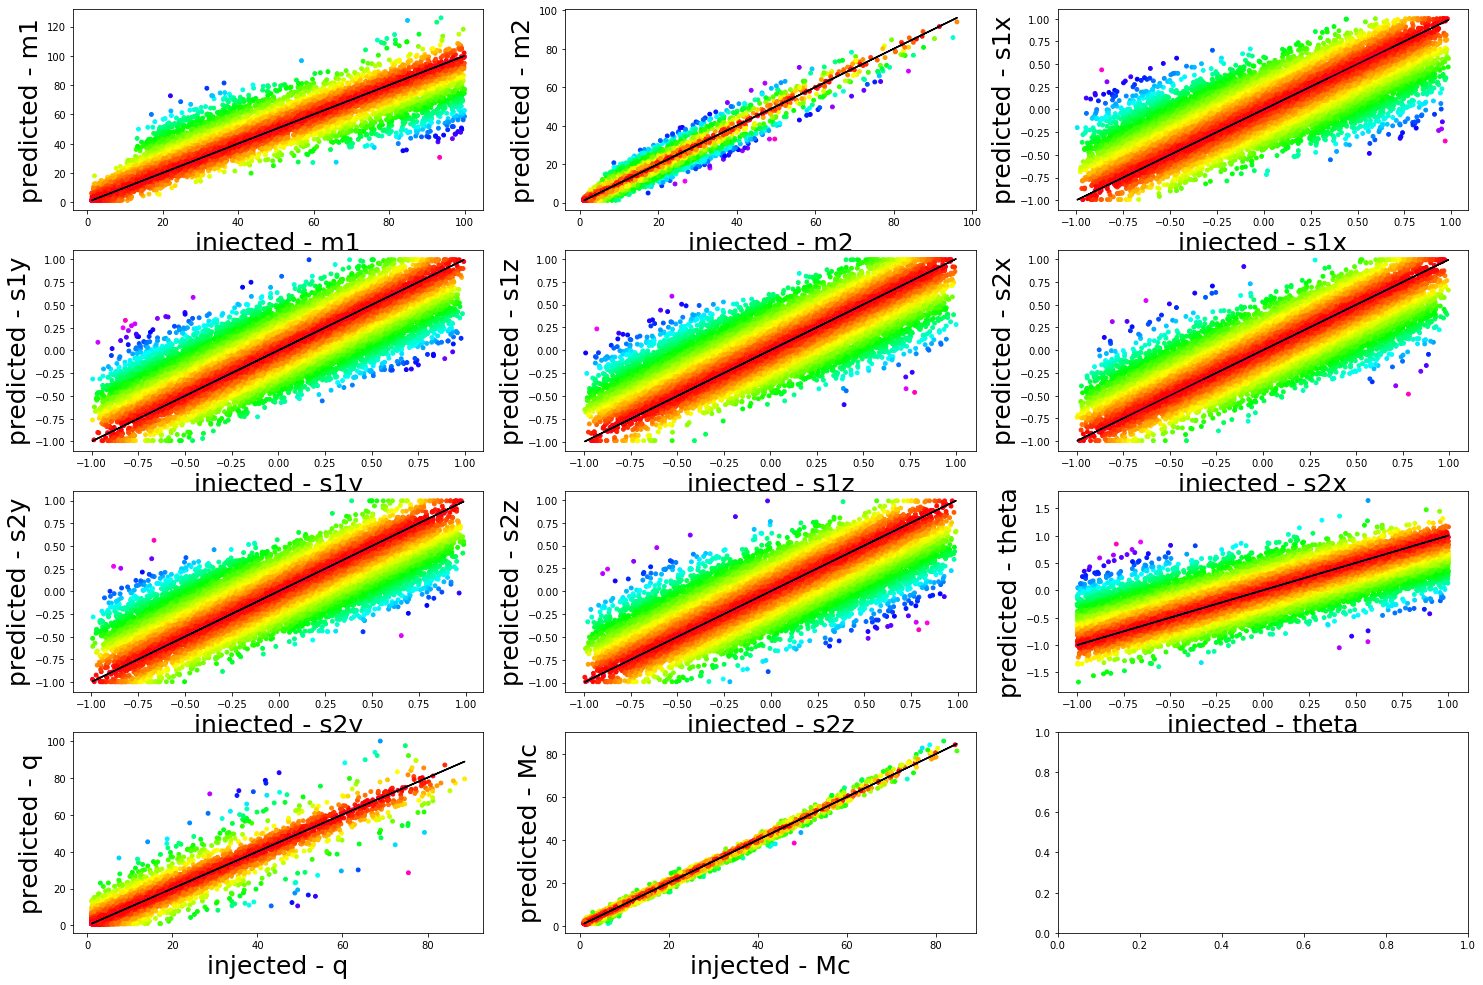
\includegraphics[width=0.45\textwidth]{./Figs/v1c0_regression.png}\\
  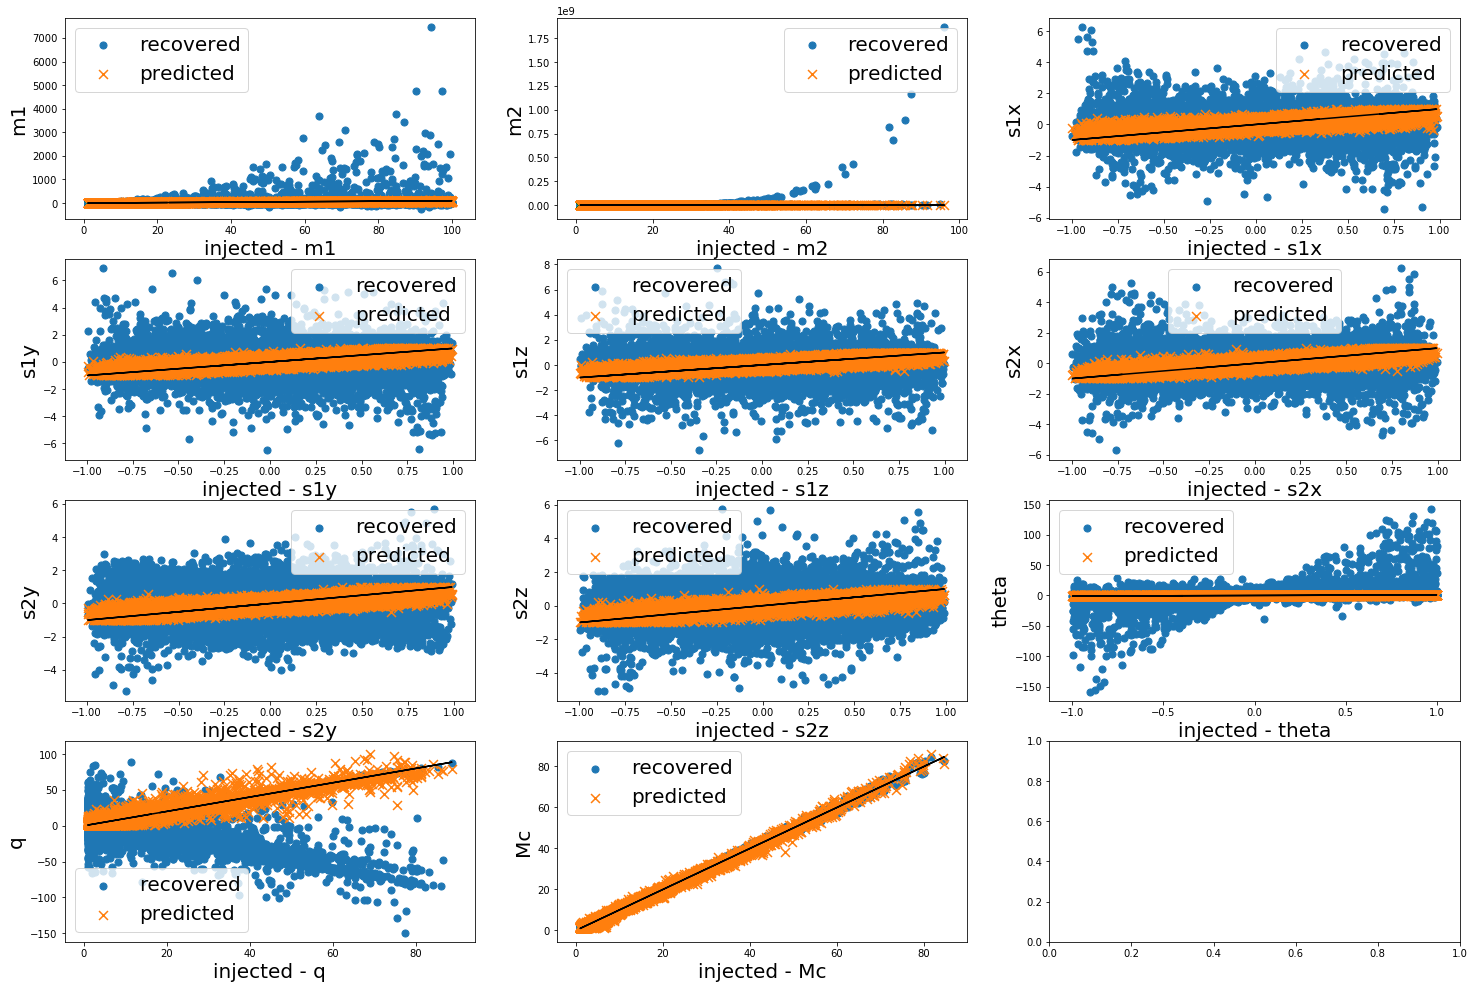
\includegraphics[width=0.45\textwidth]{./Figs/v1c0_regression_noise.png}
  \caption{\label{fig:v1c0_results} Results of the regression on the \texttt{v1c0}
  dataset. We used 2 hidden layers with 100 neurons, $N_{\rm batch}=64$, 250 epochs,  
  constrained output. See Sec.~\ref{sec:some_results} for discussion.
  The colors in the first plots is related to the absolute difference between predicted 
  and injected. The black line is the bisector.}
\end{figure}
%

%==========================================================
\subsection{Cross validation on layers}
%==========================================================
\label{sec:crossval}
In order to decide the architecture to use I did a cross validation on the 
\texttt{v0c0} dataset (the reason why I have not cross-validated on the \texttt{GstLAL} dataset
is explained in Sec.~\ref{sec:GstLAL}). I trained the models on 250 epochs using
$N_{\rm batch}=128$ for different architectures. The results are shown 
in Fig.~\ref{fig:crossval_v0c0}. The plots show that NNs with 2 layers with $\sim 100$ 
neurons each provide good enough scores and more complex NNs do not provide much better results. 
After a certain number of trainable parameters the $R^2$ coefficient reaches a plateaux 
and doesn't increase any more. 
The only exceptions are: (i) $M_c$: the best score is obtained with single-layer NNs 
(the recovered quantity is obtained only adding random Gaussian noise); 
(ii) $\theta$: this is the quantity with lowest score and the $R^2$ coefficient 
continues to (slightly) increase without reaching a plateaux even for $\sim 300$
neurons in each layer. 

Finally note that many NNs have more parameters than training samples, 
$N_{\rm param}>N_{\rm train}$, since 
$N_{\rm train}=2\cdot 10^4$ for the \texttt{v0v0} dataset. This shouldn't be a problem 
for NN (and indeed the score is good also on the test-set that has 
$N_{\rm test}=1.5\cdot 10^4$), however we could also decide to use smaller NNs 
since the accuracy in more complex NNs is not drastically better than in simpler models. 
For example in Fig.~\ref{fig:v0c0_results} and Fig.~\ref{fig:v1c0_results} I used
two hidden layers with 100 neurons so that $N_{\rm param}=12411<N_{\rm sample}=2\cdot 10^4$.

%
\begin{figure*}[]
  \center
  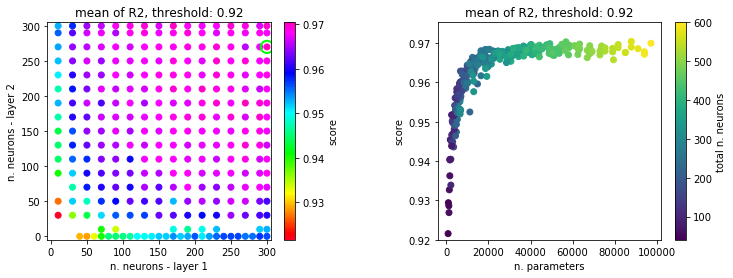
\includegraphics[width=0.45\textwidth]{./Figs/crossval_v0c0_R2mean.png}
  \hspace{0.3cm}
  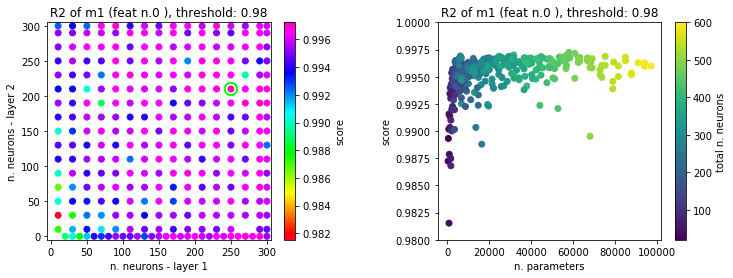
\includegraphics[width=0.45\textwidth]{./Figs/crossval_v0c0_R2m1.png} \\
  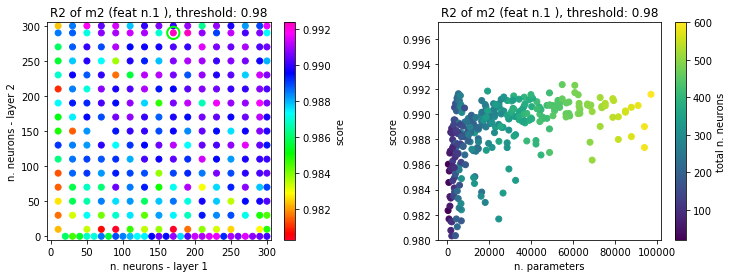
\includegraphics[width=0.45\textwidth]{./Figs/crossval_v0c0_R2m2.png}
  \hspace{0.3cm}
  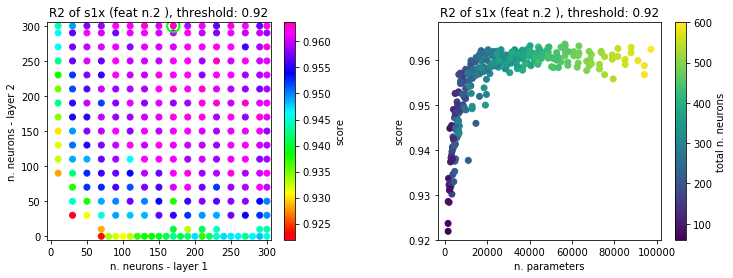
\includegraphics[width=0.45\textwidth]{./Figs/crossval_v0c0_R2s1x.png} \\
  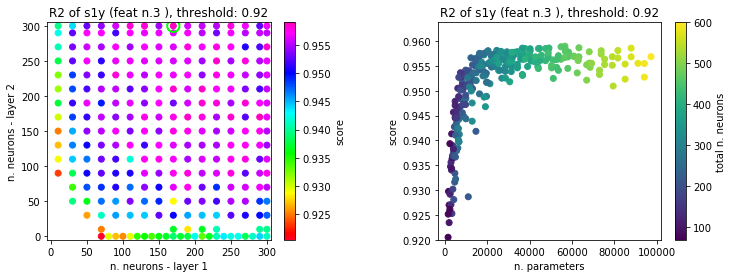
\includegraphics[width=0.45\textwidth]{./Figs/crossval_v0c0_R2s1y.png}
  \hspace{0.3cm}
  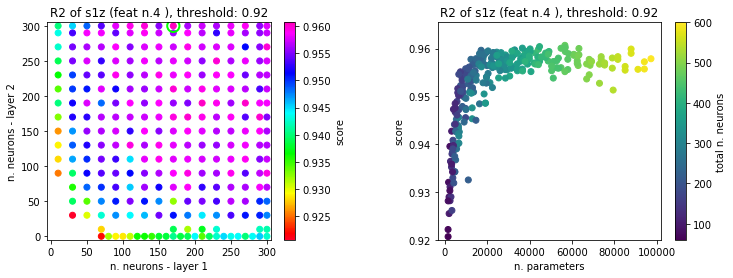
\includegraphics[width=0.45\textwidth]{./Figs/crossval_v0c0_R2s1z.png} \\
  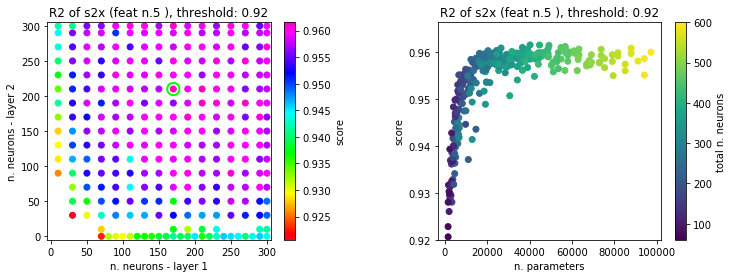
\includegraphics[width=0.45\textwidth]{./Figs/crossval_v0c0_R2s2x.png} 
  \hspace{0.3cm}
  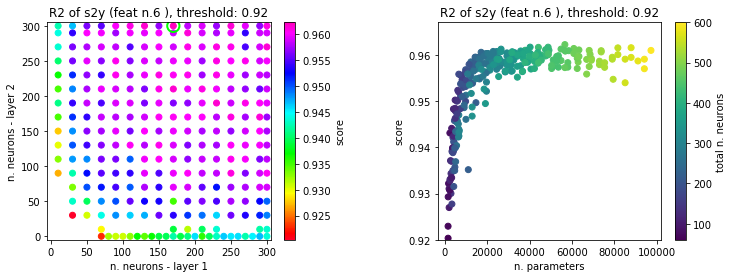
\includegraphics[width=0.45\textwidth]{./Figs/crossval_v0c0_R2s2y.png} \\
  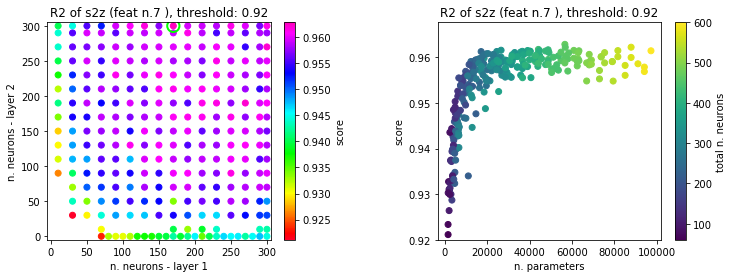
\includegraphics[width=0.45\textwidth]{./Figs/crossval_v0c0_R2s2z.png} 
  \hspace{0.3cm}
  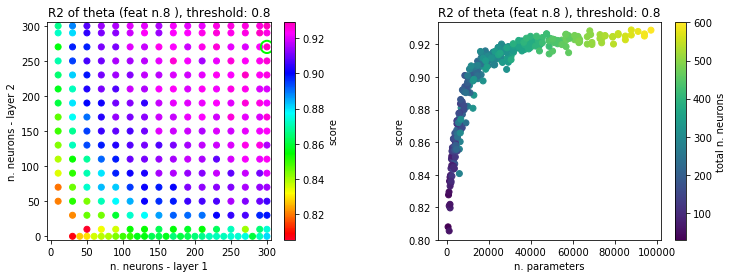
\includegraphics[width=0.45\textwidth]{./Figs/crossval_v0c0_R2theta.png} \\
  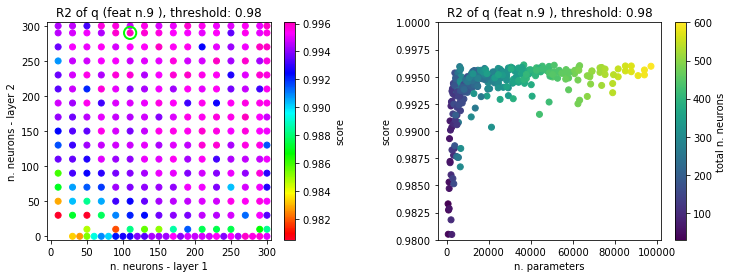
\includegraphics[width=0.45\textwidth]{./Figs/crossval_v0c0_R2q.png} 
  \hspace{0.3cm}
  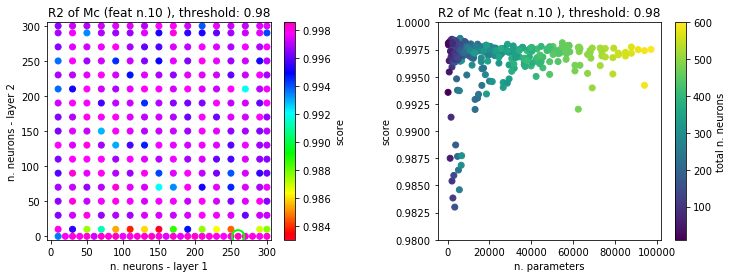
\includegraphics[width=0.45\textwidth]{./Figs/crossval_v0c0_R2Mc.png} 
  \caption{\label{fig:crossval_v0c0} $R^2$ coefficients for different architectures. 
  We show only the models that have an $R^2$ coefficient
  above the threshold indicated in the title of each panel. We show the results
  for the mean of $R^2$ and for the $R^2$ of each feature. In the rainbow-scatter plot
  the green circle marks the highest $R^2$ coefficient. }
\end{figure*}
%
\clearpage

%==========================================================
\section{GstLAL BNS dataset}
%==========================================================
\label{sec:GstLAL}
\begin{figure}[]
  \center
  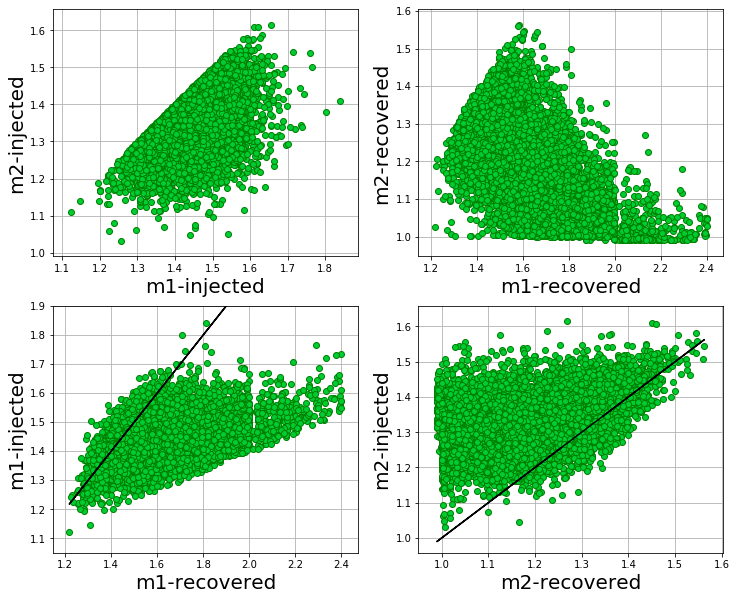
\includegraphics[width=0.45\textwidth]{./Figs/GstLAL_paperlike_m1m2.png}
  \caption{\label{fig:GstLAL_paperlike} Test-dataset, compare with Fig.1 of Chatterjee-1911.00116.}
\end{figure}

We also have a dataset obtained with injected parameters of nonspinning 
BNSs recovered with \texttt{GstLAL}.
In this case we have only three features: $m_1$, $m_2$, $M_c$.
The regression on this dataset is more problematic:
\begin{itemize}
\item The output of the regression for the two masses $m_i$ seems almost independent on the 
architecture and is not improved with more complex NNs. The result for $M_c$ instead is 
more sensible on the architecture (but the regression seems useless for $M_c$)

\item The predictions of $m_i$ have a sharp edge in correspondence of the region with 
most degeneracy, see Fig.~\ref{fig:GstLAL_results}

\item The model stops to learn after the second epoch. Training for more epochs only improves
the prediction of the lowest and highest chirp masses, but does not improve the prediction
of $m_i$. 

\item The mass ratio computed with the predicted masses is in a very narrow range while
the injection have a much wider interval, see the last panel of Fig.~\ref{fig:GstLAL_results}.

\end{itemize} 

Therefore in this case the regression does not seem to work properly. I have also tried to 
do the regression only on $m_{1,2}$ and $M_c$ and recovering the other mass analytically 
but the results are the same. Even SVR gives the same results (qualitatively).
%
\begin{figure}[]
  \center
  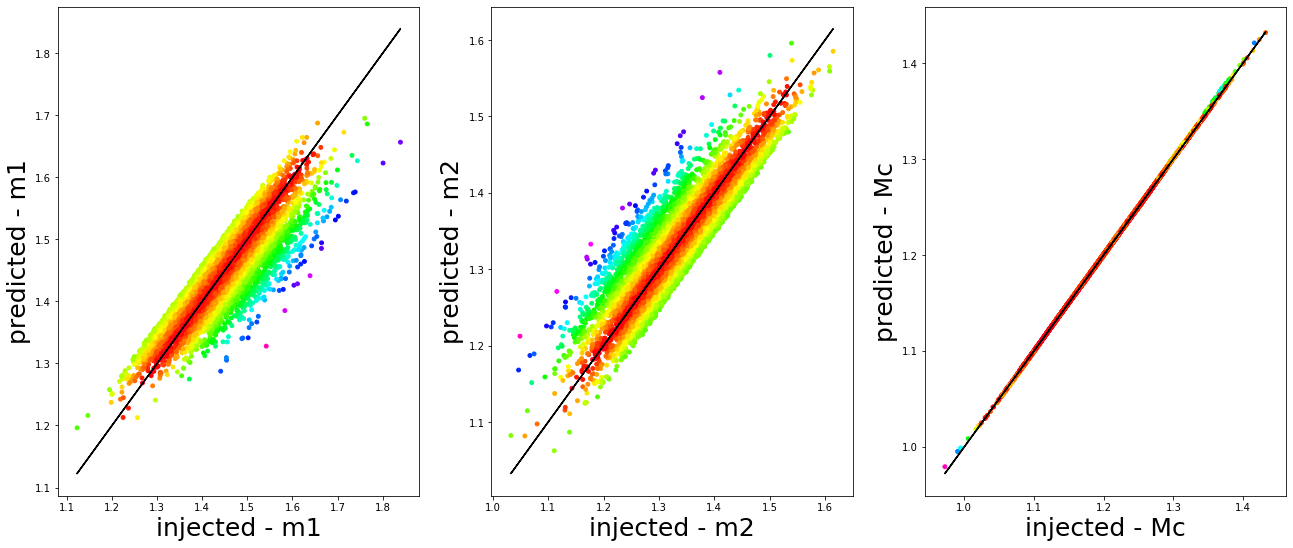
\includegraphics[width=0.47\textwidth]{./Figs/GstLAL_regression.png}
  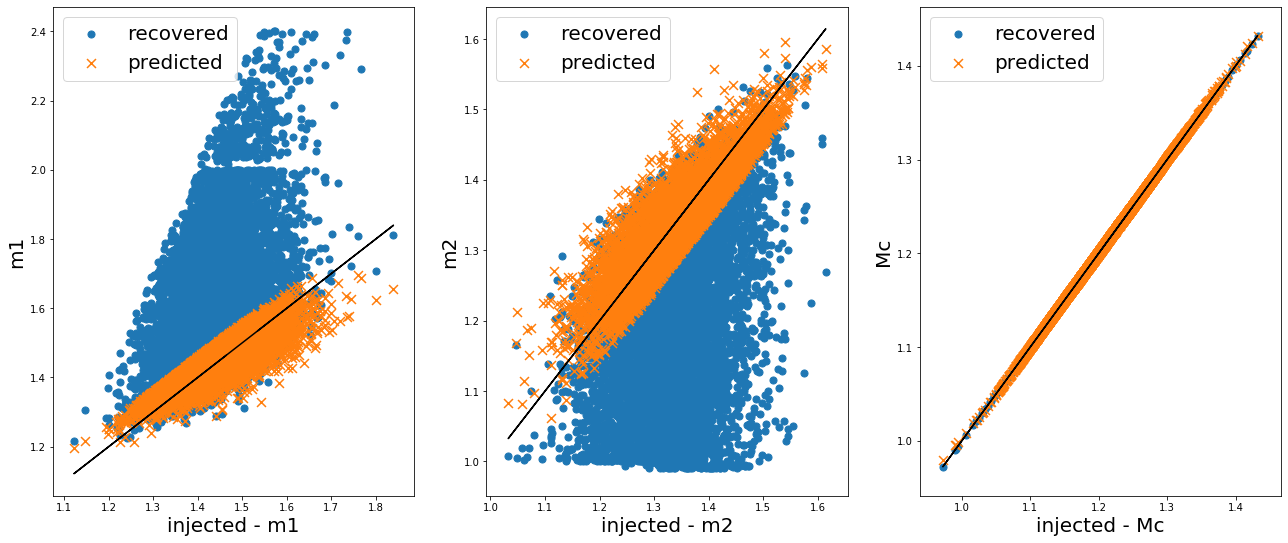
\includegraphics[width=0.47\textwidth]{./Figs/GstLAL_regression_noise.png}
  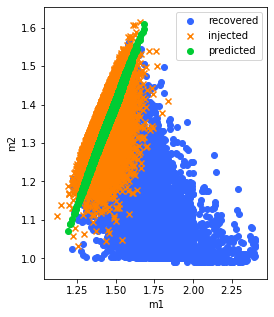
\includegraphics[width=0.15\textwidth]{./Figs/GstLAL_m2.png}
  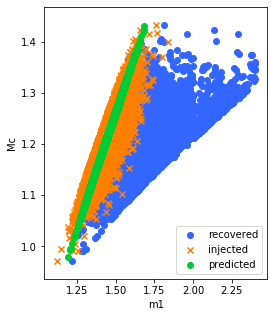
\includegraphics[width=0.15\textwidth]{./Figs/GstLAL_Mc.png}
  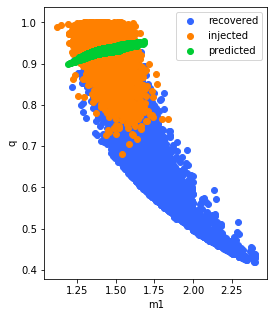
\includegraphics[width=0.15\textwidth]{./Figs/GstLAL_q.png}
  \caption{\label{fig:GstLAL_results} Results of the regression on the \texttt{GstLAL}
  dataset. We used one hidden layer with 100 neurons, $N_{\rm batch}=64$, 50 epochs,  
  unconstrained output.
  The colors in the first plots is related to the absolute difference between predicted 
  and injected. The black line is the bisector.
  The final $R^2$ coefficients for $m_1$, $m_2$ and $M_c$ 
  are 0.7363, 0.7819, and 0.9999, respectively.
  In the last three panels we plot $m_2$, $\Mc$ and $q$ over $m_1$ for the injected, recovered
  and predicted quantities.}
\end{figure}

%==========================================================
\subsection{Loss function, attempt 1}
%==========================================================
\label{sec:loss}
In order to fix the problem with $q$ in the \texttt{GstLAL} dataset, 
I tried to modify the loss function to minimize.
The default function for regression tasks is the Mean Squared Error
\begin{equation}
J_{\rm mse} = {\rm mean} \sum_i \left( y^{\rm true}_i - f(x_i) \right)^2 .
\end{equation}
I tried to modify it including a $q$-penalty and a $\Mc$-penalty:
\begin{align}
J =  {\rm mean} & \left(  \sum_i \left( y^{\rm true}_i - f(x_i) \right)^2 \right.   \nonumber \\
&  + \lambda_{\rm q} \sum_i \left( q^{\rm true}_i - q^{\rm pred}_i \right)^2
\nonumber \\
& \left. + \lambda_{\rm \Mc} \sum_i \left( M_{c,i}^{\rm true} - M_{c,i}^{\rm pred} \right)^2 \right)
\end{align}
where (not surprisingly)
\begin{align}
q^{\rm pred}_i &  = \frac{m_{2,i}^{\rm pred}}{m_{1,i}^{\rm pred}}, \\
M_{c,i}^{\rm pred} & = 
\frac{\left(m_{1,i}^{\rm pred}m_{2,i}^{\rm pred} \right)^{3/5}}{\left(m_{1,i}^{\rm pred}+m_{2,i}^{\rm pred}\right)^{1/5}},
\end{align}
and $q^{\rm true}$, $\Mc^{\rm true}$ are analogous. Note the $\Mc$-term is not the same 
in MSE since here the chirp mass is computed using $m_i$ while in the MSE part $\Mc$ 
is the third feature.
In order to have the predicted masses in the loss function we need to 
rescale $x$ but since the loss function is defined using the Keras backend and 
for the moment this is implemented only for  \texttt{MinMaxScaler}. 
We cannot use \texttt{numpy} in the Keras backend, so the loss function is not fully vectorized
(but this is not a big issue). 
I tried to fit the data with different values for the hyperparameters $\lambda_q$ and
$\lambda_Mc$ but in every case I didn't find a solution to the issues of Sec.~\ref{sec:GstLAL}
since the effect of these penalty is marginal, even if we use high values for $\lambda_i$.
Maybe this is not the correct way to include penalties. 

%==========================================================
\subsection{GstLAL BNS dataset - a different approach}
%==========================================================
\label{sec:GstLAL2}
%
\begin{figure}[]
  \center
  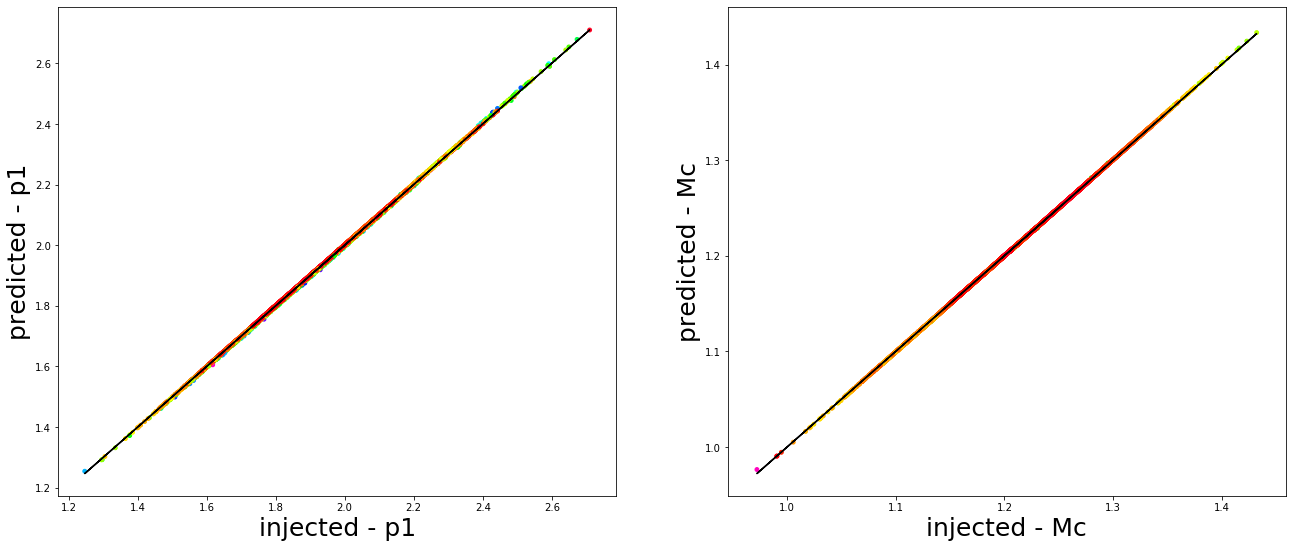
\includegraphics[width=0.43\textwidth]{./Figs/GstLAL_p_regression.png}
  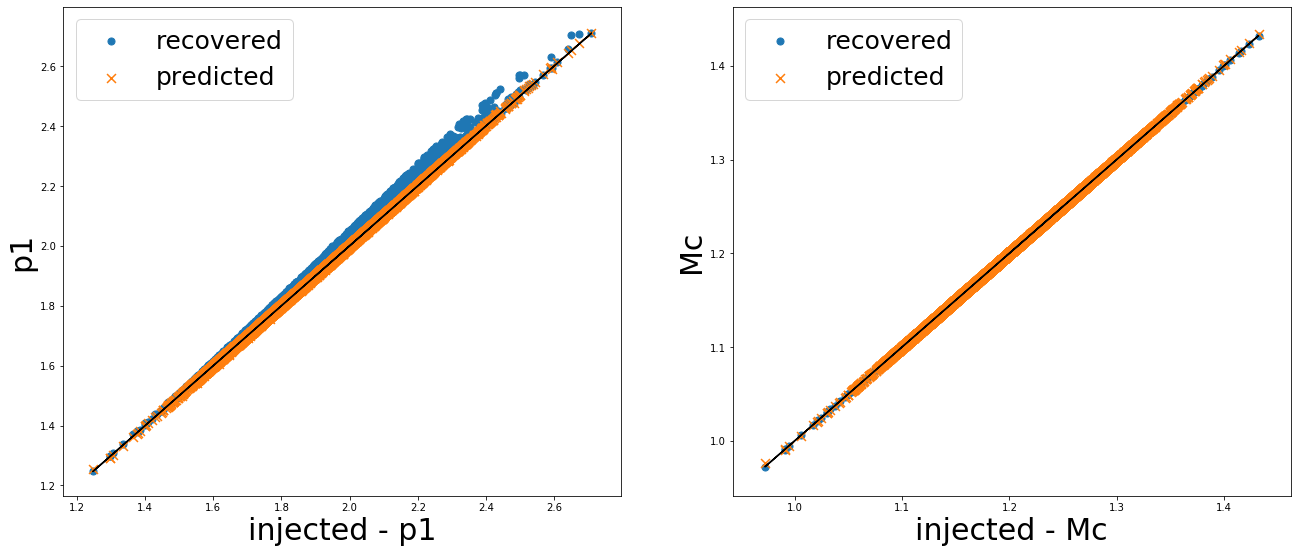
\includegraphics[width=0.43\textwidth]{./Figs/GstLAL_p_regression_noise.png}\\
  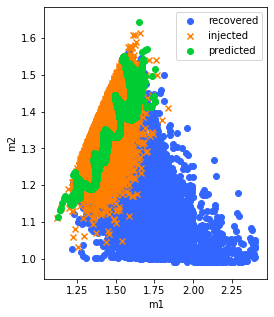
\includegraphics[width=0.15\textwidth]{./Figs/GstLAL_p_m2.png}
  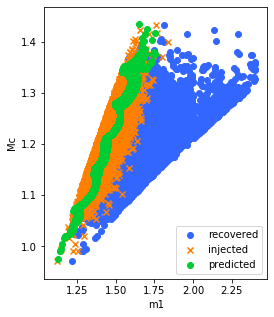
\includegraphics[width=0.15\textwidth]{./Figs/GstLAL_p_Mc.png}
  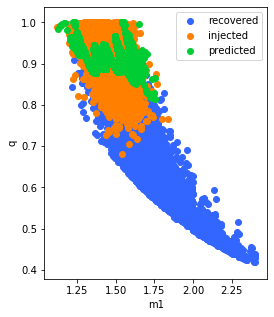
\includegraphics[width=0.15\textwidth]{./Figs/GstLAL_p_q.png}\\
  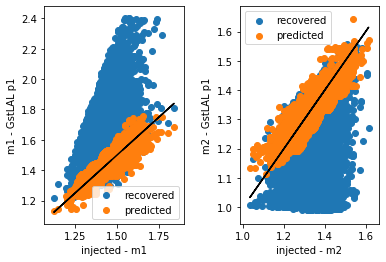
\includegraphics[width=0.22\textwidth]{./Figs/GstLAL_p_m1m2.png}
  %\hspace{0.3cm}
  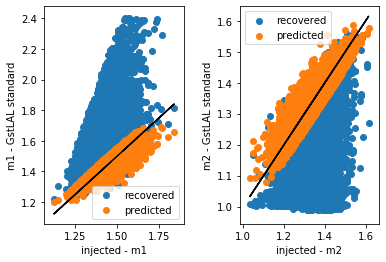
\includegraphics[width=0.22\textwidth]{./Figs/GstLAL_standard_m1m2.png}
  \caption{\label{fig:GstLAL2_results} Results of the regression on the \texttt{GstLAL}
  dataset using the approach of Sec.~\ref{sec:GstLAL2}. 
  We used one hidden layer with 100 neurons, $N_{\rm batch}=128$, 100 epochs,  
  unconstrained output.
  The colors in the first plots is related to the absolute difference between predicted 
  and injected. The black line is the bisector.
  The final $R^2$ coefficients for $p=m_1 m_2$ and $\Mc$ are 0.99993 and 0.99997,
  respectively.
  In the three panels in the middle we plot $m_2$, $\Mc$ and $q$ over $m_1$ for 
  the injected, recovered and predicted quantities.
  Finally, in the first two panels of the last row we show the (indirectly) predicted masses 
  with the ($p$, $\Mc$) regression versus the injected masses, 
  while in the last two panels of the last row we show the 
  predicted masses obtained with the standard regression of Sec.~\ref{sec:GstLAL} versus 
  the injected ones.}
\end{figure}
%
I also tried to do something different on the \texttt{GstLAL} dataset. 
So the pipeline recovers $\Mc$ perfectly (I am not even sure that make a regression on $\Mc$
makes sense), then I suppose that it recovers also one of the two masses 
(I don't know which one) and compute the second one analytically. Therefore the degeneracy problem
in one mass should be "specular" in the other masse, so maybe to remove the degeneracy problem
in the regression we can consider suitable combinations of the two masses $m_i$ instead of 
considering them separately. The using this quantity $g(m_1,m_2)$ and $\Mc$ we can obtain 
two masses $m_i$. It turns out that symmetric quantities are better, in particular 
$p_k= (m_1 m_2)^k$ can be regressed very well if the exponent $k$ is not too high, 
obtaining $R^2$ coefficients such that $1-R^2 \leq 10^{-4}$. Then the two masses can be
obtained analytically from
\begin{equation}
\label{eq:m12frompMc}
m_{1,2} = \frac{p^3}{2 \Mc^5}\left( 1 \pm \sqrt{1-4\nu} \right),
\end{equation}
where $p=m_1 m_2$ (i.e. we omit the index $k=1$) and $\nu$ is the symmetric mass ratio
\begin{equation}
\nu \equiv \frac{\Mc^{10}}{p^5} = \frac{m_1 m_2}{(m_1+m_2)^2}\in (0, \frac{1}{4}].
\end{equation}
However, note that the condition
\begin{equation}
\label{eq:nu_condition}
\nu=\Mc^{10}/p^5\leq \frac{1}{4}
\end{equation} 
is not enforced during the training (i.e. the predictions for 
$p_k$ and $\Mc$ are not constrained in this sense), 
then it is possible that~\eqref{eq:nu_condition} will be slightly violated, making
the two masses complex. For this reason we recover the two masses with a modified version
of Eq.~\eqref{eq:m12frompMc}
\begin{equation}
\label{eq:m12frompMc_mod}
m_{1,2}^{\rm pred} = \frac{p_{\rm pred}^3}{2 M_{c, \rm pred}^5}\left( 1 \pm \sqrt{1-4 \min\left(\nu_{\rm pred}, \frac{1}{4}\right)} \right).
\end{equation}
Note that the condition~\eqref{eq:nu_condition} can be violated pretty often 
if we have many equal-mass binaries in the dataset (and this is precisely our case).
However note that with this approach the predictions for $m_i$ and $\Mc$ can be not
consistent, i.e. 
$\Mc^{\rm pred} \neq (m_1^{\rm pred} m_2^{\rm pred})^{3/5}/(m_1^{\rm pred} + m_2^{\rm pred})^{1/5}$.
To enforce this condition we then compute $m_2^*$ requiring 
\begin{equation}
\Mc^{\rm pred} \equiv \frac{(m_i^{\rm pred} m_j^*)^{3/5}}{(m_i^{\rm pred} + m_j^{*})^{1/5}},
\end{equation}
where $i\neq j=1,2$, explicitly (omitting the superscript 'pred' in the RHSs):
\begin{align}
m_j^* &= \frac{\Mc^{5/3}\left(3^{1/3} 2 \Mc^{5/3}+2^{1/3} S_i^2 \right) }{ 6^{2/3} m_i^{3/2} S_i },  \\
S_i   &= \left(9 m_i^{5/2} + \sqrt{81 m_i^5 -12 \Mc^5}\right)^{1/3}.
\end{align}

The results for this kind of regression using the features $p=m_1 m_2$ and $\Mc$
are shown in Fig.~\ref{fig:GstLAL2_results}. We use a NN with one hidden layer with 
100 neurons and ReLU, linear activation function in the output layer (i.e. no constraints),
MSE loss function and we train for 100 epochs using $N_{\rm batch}=128$. 
While the regression on $p$ and $\Mc$ is almost perfect ($R^2$ coefficients of 0.99993 and 
0.99997, respectively), the other recovered quantities show some strange behavior and, most
importantly, they are strongly dependent on the initial state on the NN, i.e. training the NN
different times using always the same options leads to pretty different results for $m_i$ and $q$.
Moreover, the mean predicted/injected errors for $m_1$, $m_2$, $\Mc$, and $q$ are slightly worse 
since here we get $2.8\%$, $2.7\%$, $0.02\%$, and $5.4\%$ respectively, while with the standard 
regression of Sec.~\ref{sec:GstLAL} we got $2.3\%$, $2.2\%$, $0.05\%$ and $4.6\%$.

Another attempt could be to do the regression on $\nu$ and $\Mc$ and then compute $m_i$
from these two quantities. 
In this case we could apply a constrained output function to $\nu$  in order to have a more
consistent output
(and in this case we should write a new class for the linear-scaler since the 
\texttt{MinMaxScaler} that we are using now in the constrained output wouldn't be the best 
choice for constraining a quantity like $\nu$). 
However I don't think that this will solve all the problems that we have
with this dataset.

%==========================================================
\subsection{GstLAL BNS dataset - the return of the different approach}
%==========================================================
\label{sec:GstLAL3}
%
\begin{figure}[]
  \center
  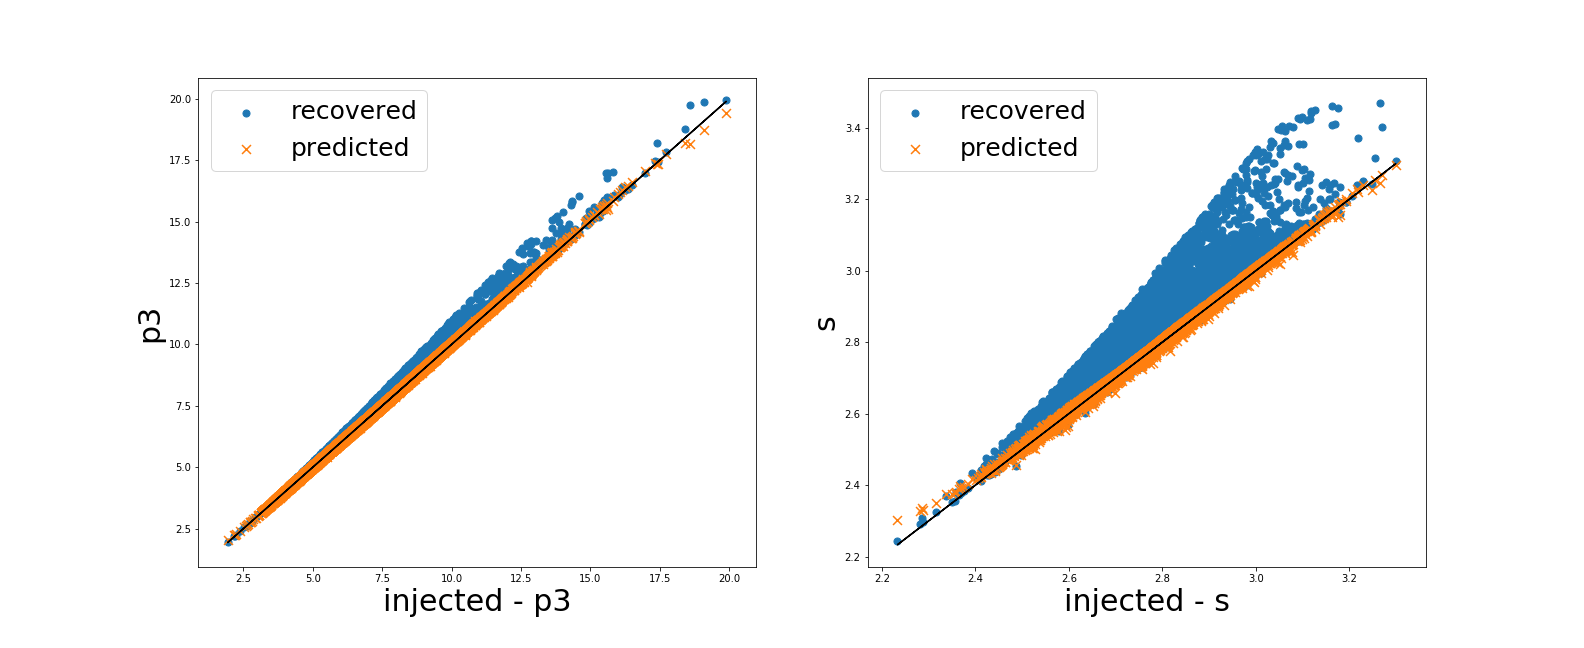
\includegraphics[width=0.48\textwidth]{./Figs/80_resultReg}\\
  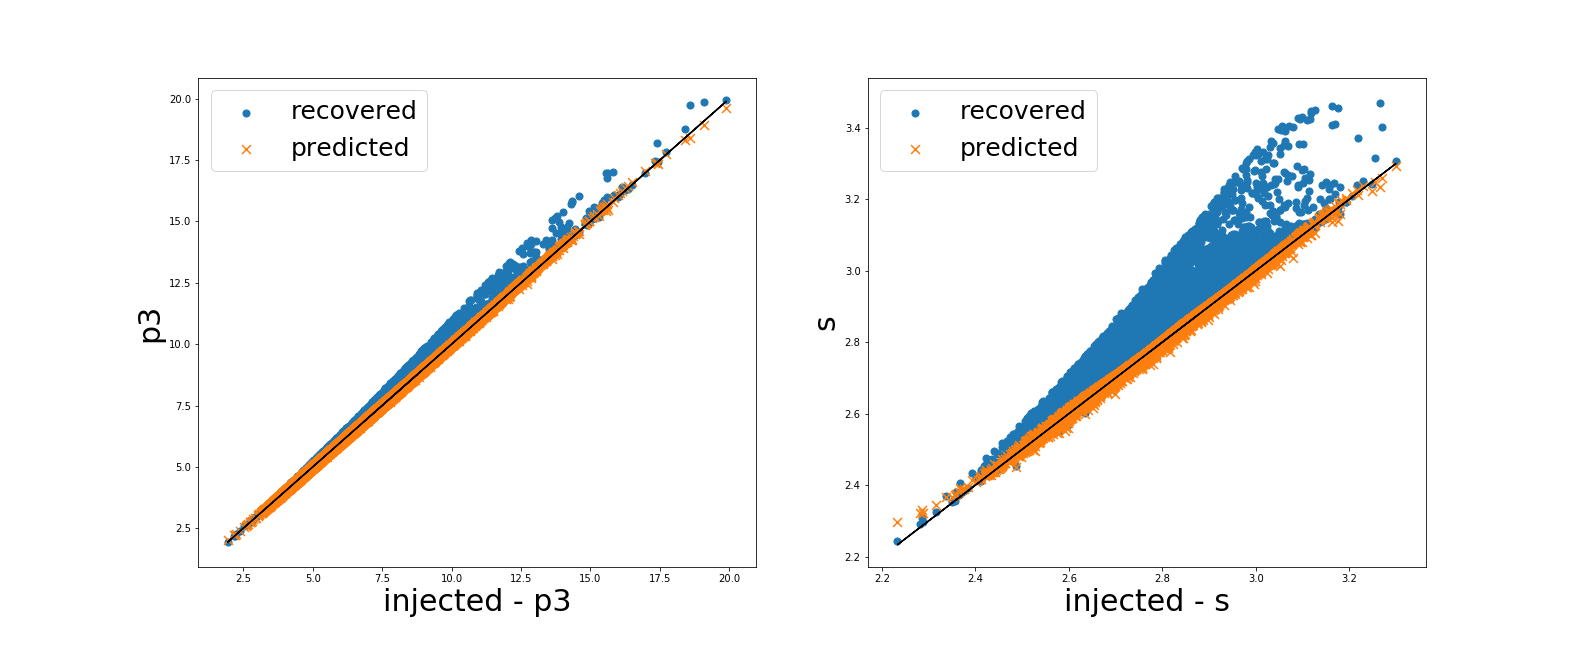
\includegraphics[width=0.48\textwidth]{./Figs/100_resultReg}\\
  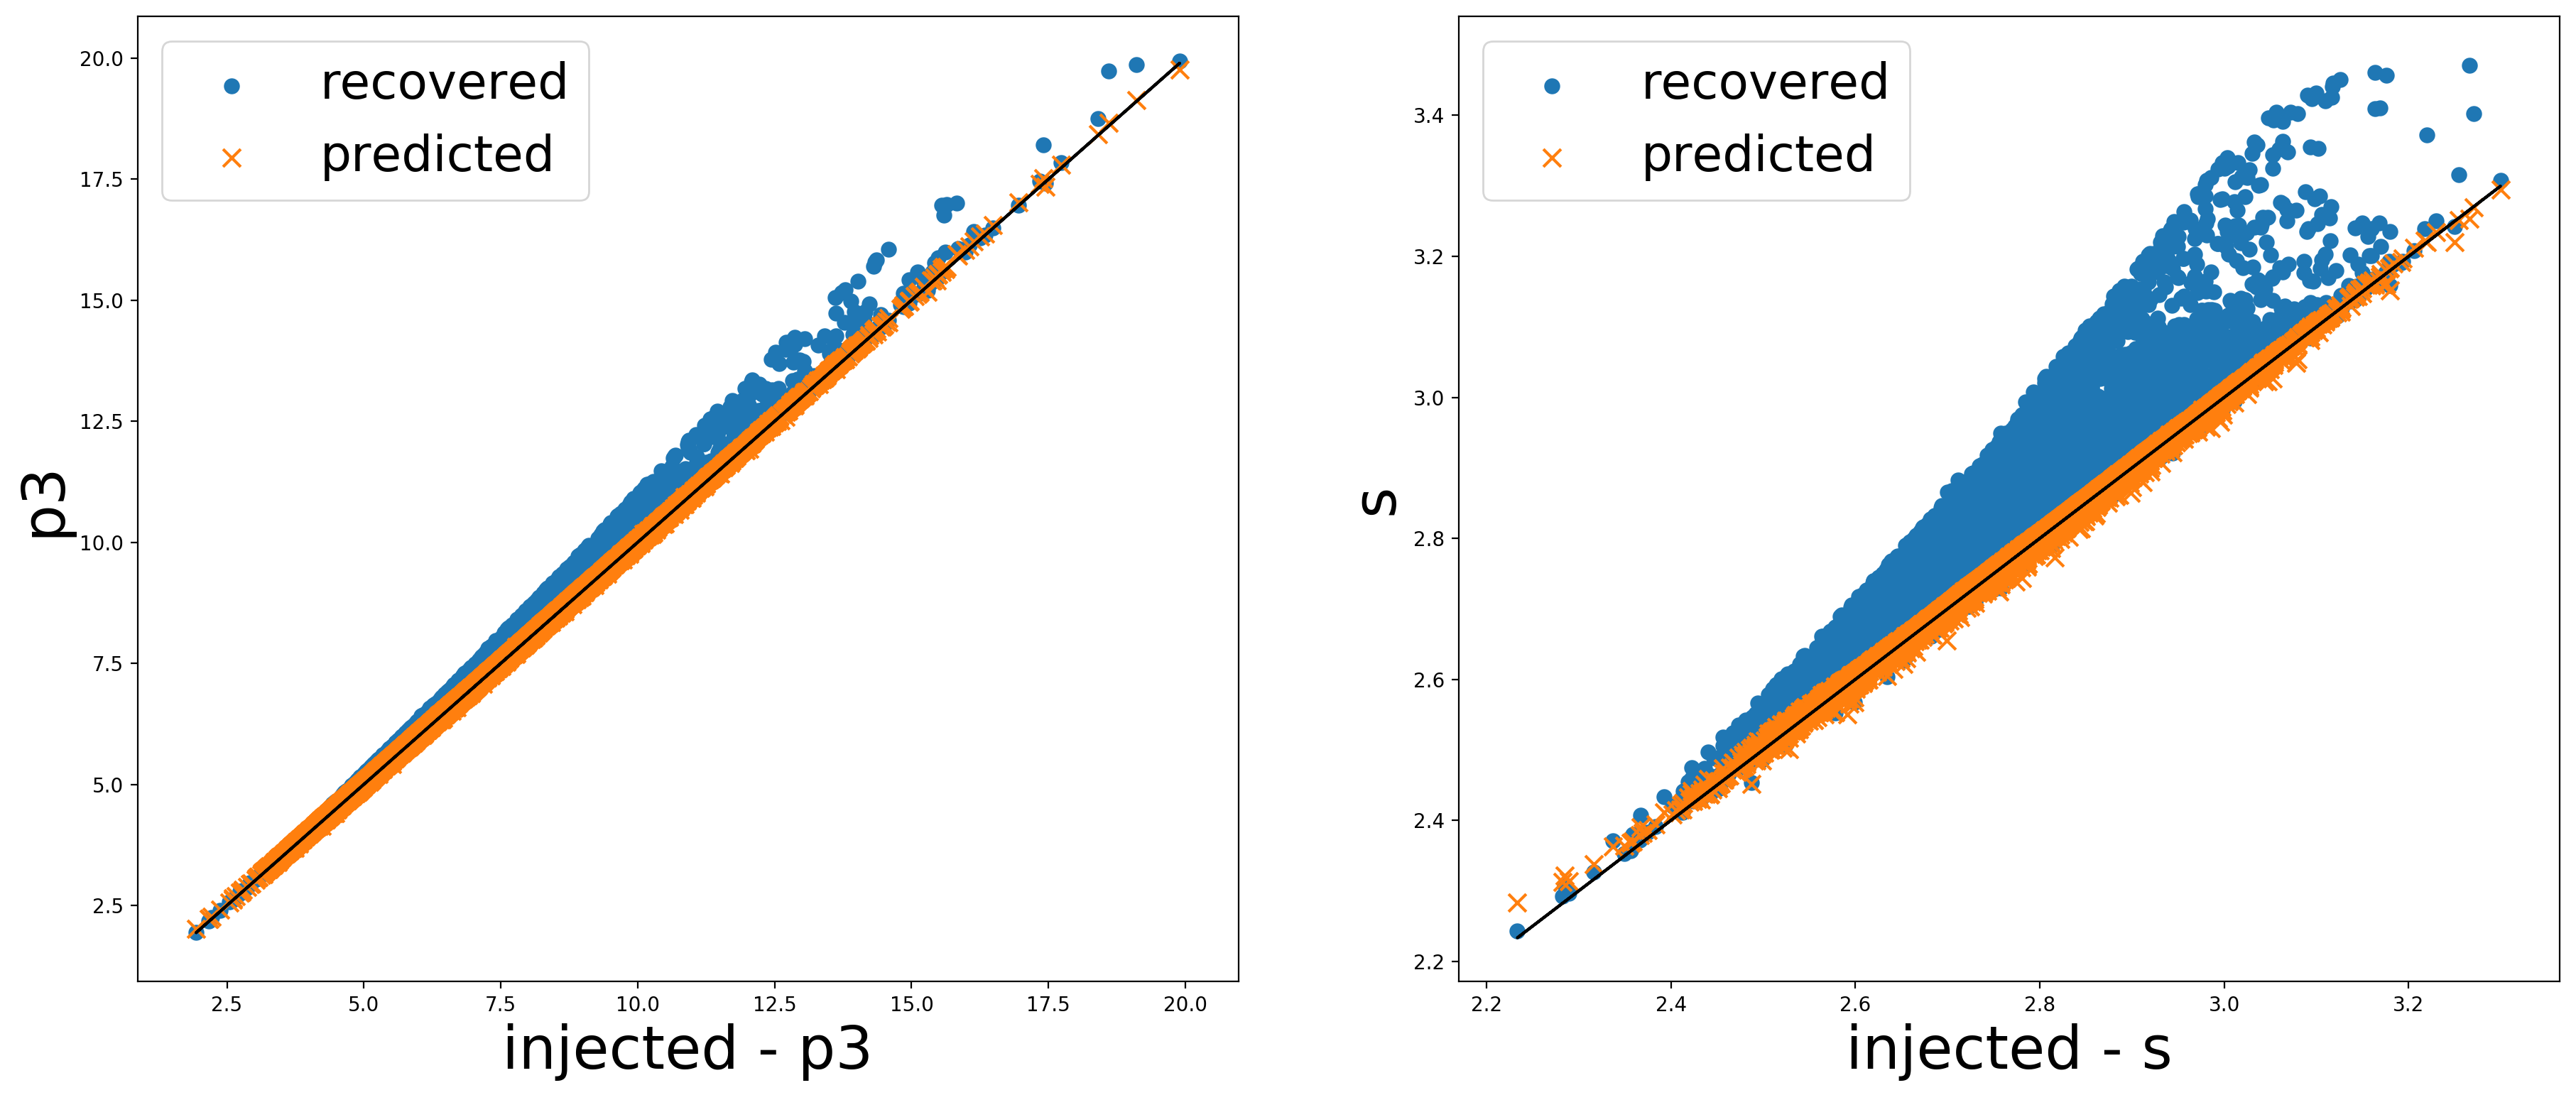
\includegraphics[width=0.43\textwidth]{./Figs/290_}
  \caption{\label{fig:approach3_comparison1} Results from the regression 
  for 80, 100 and 290 hidden layers top to bottom, with approach (s,p).}
\end{figure}
%
\begin{figure*}[]
  \center
  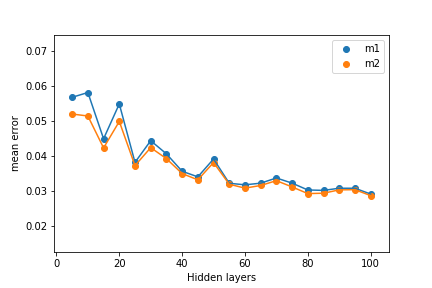
\includegraphics[width=0.32\textwidth]{./Figs/merrorwlayers}
  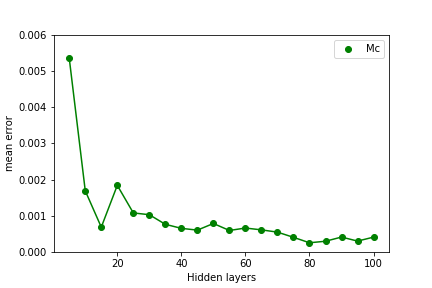
\includegraphics[width=0.32\textwidth]{./Figs/mcerrorwlayers}
  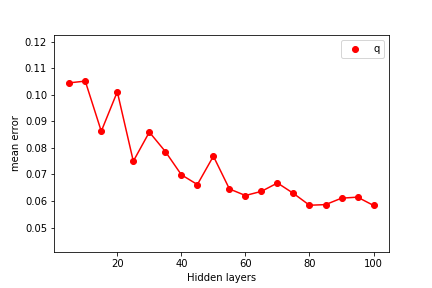
\includegraphics[width=0.32\textwidth]{./Figs/qerrorwlayers}
  \caption{\label{fig:error_with_layers} Errors obtained for different hidden layer size using the regression data $p$ and $s$ from Sec. \ref{sec:GstLAL3}}
\end{figure*}
%
Marina thinks (hello) that using different variables constructed from $m_1$ and $m_2$ may be a good approach, along the modified loss function to add information without regressing more variables. Also it is true that a NN constructs within new variables that are (non)linear combinations of the input ones, so ideally the NN should do that step for us. Guessing that it does not do so, I propose the following:

Instead of considering just one \textit{made-up} quantity, let's consider two such that
\begin{equation}
p=(m_1m_2)^3 \hspace{1cm} s=m_1+m_2.
\end{equation} 

The idea behind this definition is that the known chirp mass then would be $\mathcal{M}_c=(p/s)^{1/5}$, and we aim to reduce the degeneracy. Once these variables are regressed, the original masses can be recovered by
\begin{equation}
m_1=\frac{s+\sqrt{s^2-4\sqrt[3]{p}}}{2} \hspace{1cm} m_2=s-m1.
\end{equation}

If we analyze the content of the square root we can see that $s^2-4\sqrt[3]{p}=(m_1+m_2)^2-4m_1m_2=(m1-m_2)^2$ and therefore it would be always positive. This is also why we take its the positive sign. In practice and as the regression is not perfect, the content of the square root can be slightly negative $(\mathcal{O}(10^{-3})$, and then we will take it as zero and both masses would be equal. With this definition there are no conditions of further restrictions.

For the moment, we consider the loss function just \textit{MSE}. Training with 20 epochs, more than enough to saturate the training, we try with different number of hidden layers getting the mean errors that can be seen in figure \ref{fig:error_with_layers}. All the quantities reduce the error with the number of layers but in an oscillatory way. For this study, the minimum error is obtained with 290 layers.

Then we compare results for 80, 100 and 290 hidden layers in figures  \ref{fig:approach3_comparison1}-\ref{fig:approach3_comparison3}. We use these two lower numbers to illustrate how a NN with less parameters behave, and then the optimal one from the nets tried. All  obtain a high accuracy in the computed parameters ($>0.99$). 

Some tests where implemented to control the behaviour of the predicted masses from the parameters $s$ and $p$ proposed: first we control that mass1 is always below the threshold of 3 solar masses to consider it a NS. 

Then we can recover mass2 either from the injected chirp mass or from the algebraic relation using $s$ and $m_1$. So we calculate the difference of the values obtained through these two methods, and show a warning if the difference is bigger than 0.02 (arbitrary reasonably low number). We never get an alert, and some examples of the errors obtained can be seen in figure \ref{fig:approach3_comparison2}.

Finally in figure \ref{fig:approach3_comparison3} we compare the recovered, injected and predicted values for $m_2$, $\mathcal{M}_c$ and $q$ as a function of $m_1$. We can see that the predicted values are always over the region of injected values, and not in the region of wrongly recovered ones; I would suggest this is good. But during an interval of $m_1$ it covers a narrower parameter space that it should. Also it is curious that with 80 and 290 layers we have a very similar behaviour in the plots, but with 100 the results look better.  My theory: for $m_1\in(1.5,1.75)$ and mass ratio $q<0.9$ (approximate values from the plots) the regression is more difficult. So when we have less layers the error is bigger, then there is an appropriate number of layers around 100 that performs the best. And finally a very high number of layers overfits the data in the ``easier" region getting a better score, but performs equally bad in the complicated region.
%
\begin{figure}[]
  \center
  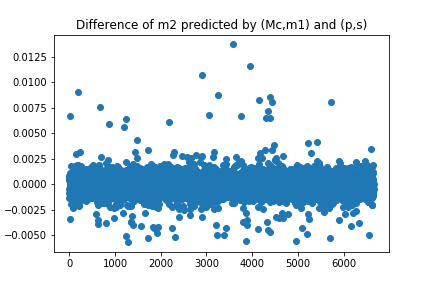
\includegraphics[width=0.23\textwidth]{./Figs/80_m2_dif}
  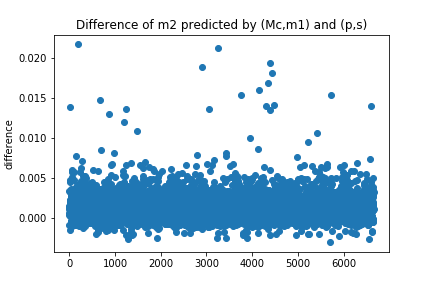
\includegraphics[width=0.23\textwidth]{./Figs/100_m2_dif}
  \caption{\label{fig:approach3_comparison2} Difference between two ways of obtaining mass2 for 80 hidden layers (left) and 100 (right) with approach (s,p).}
\end{figure}
%
\begin{figure}[]
  \center
  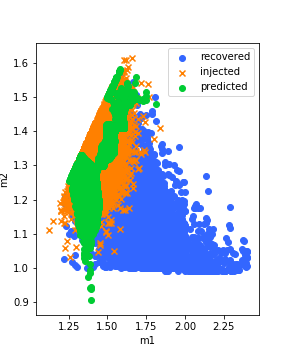
\includegraphics[width=0.15\textwidth]{./Figs/80_masses}
  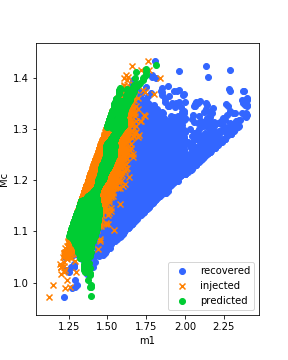
\includegraphics[width=0.15\textwidth]{./Figs/80_Mc}
  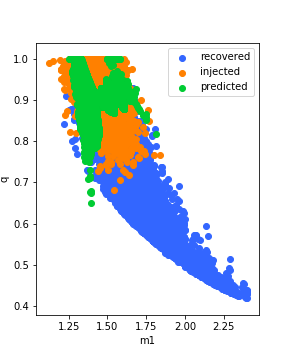
\includegraphics[width=0.15\textwidth]{./Figs/80_q}
  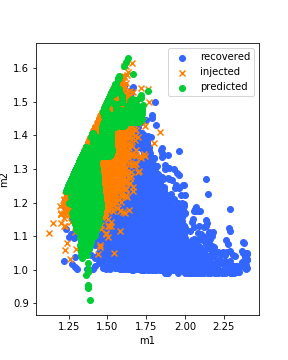
\includegraphics[width=0.15\textwidth]{./Figs/100_masses}
  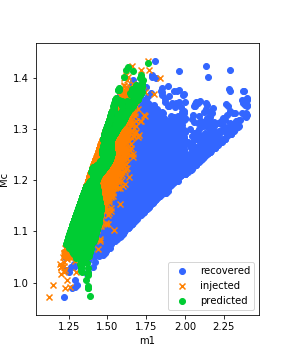
\includegraphics[width=0.15\textwidth]{./Figs/100_Mc}
  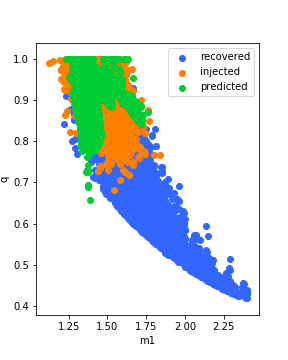
\includegraphics[width=0.15\textwidth]{./Figs/100_q}
  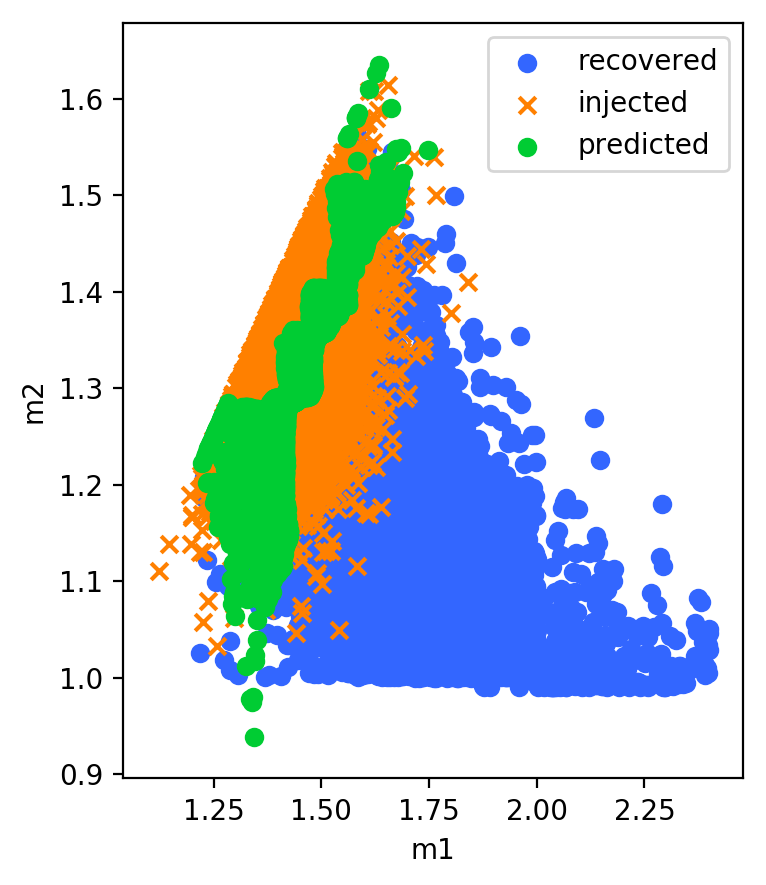
\includegraphics[width=0.15\textwidth]{./Figs/290_m1m2all}
  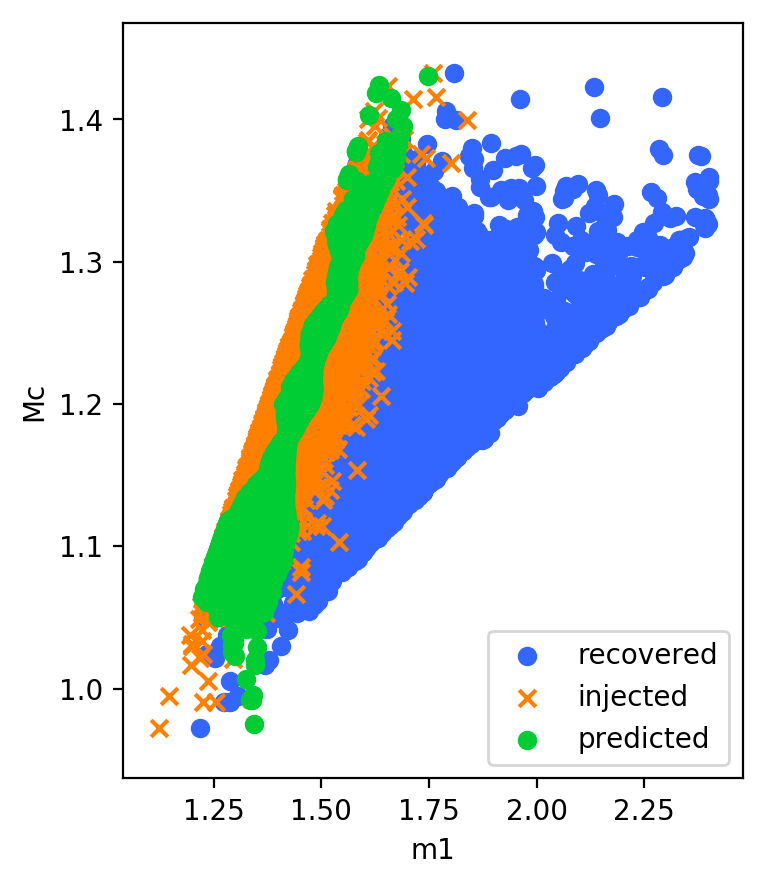
\includegraphics[width=0.15\textwidth]{./Figs/290_m1Mcall}
  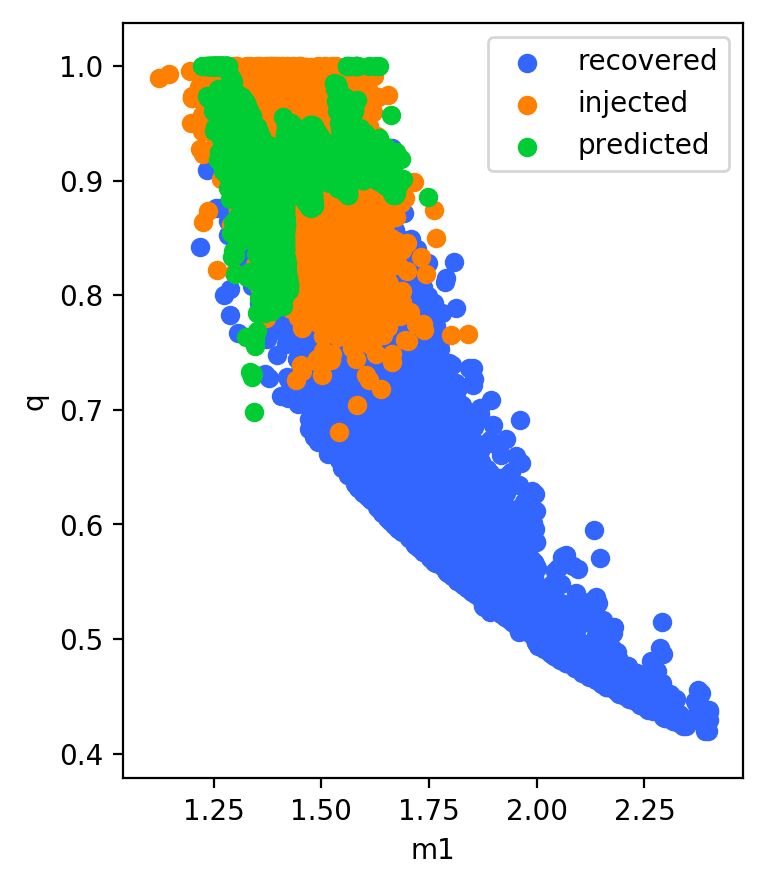
\includegraphics[width=0.15\textwidth]{./Figs/290_q}
  \caption{\label{fig:approach3_comparison3} predicted vs recovered vs injected quantities, 80, 100 and 290 hidden layers top to bottom, with approach (s,p).}
\end{figure}
%
%==========================================================
\subsection{The loss-function strikes back}
%==========================================================
%
\begin{figure*}[]
  \center
  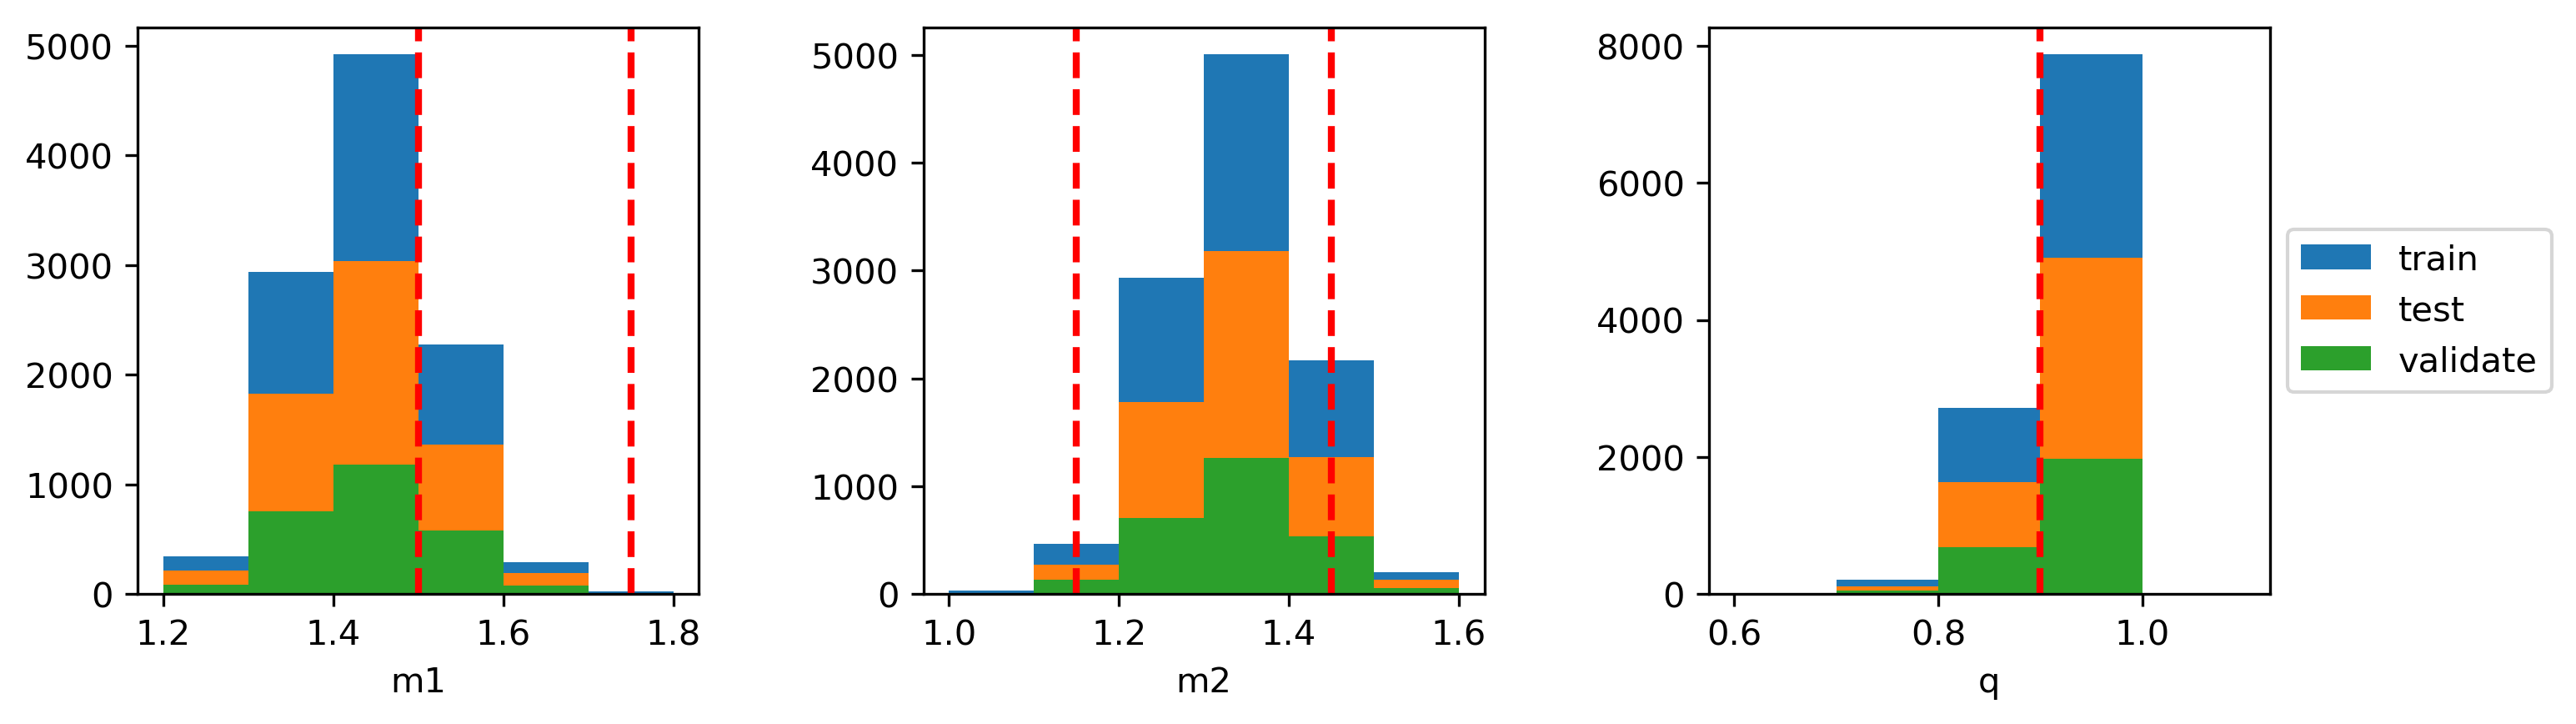
\includegraphics[width=0.95\textwidth]{./Figs/hists_data}
  \caption{\label{fig:analysisGstLAL} Histograms of the data used for training, validating and testing. For the masses, the red lines enclose the problematic region, and for the mass ratio, we put the division at 0.9.}
\end{figure*}
%
\label{sec:loss_new}
The loss function is very important for the NN, but not only its value, but its shape. This is because for updating the parameters in each iteration it does a (kind of) gradient descent, so it is not only the value, but the derivative, what we have to tune. I think that the losses proposed up there are not good because of this.

I propose the loss function 
\begin{equation}
J_{\rm mse} = {\rm mean} \Bigg[ \left( \sum_i \left( y_i - \hat{y}_i \right)^2 \right) \cdot(1+\lambda(\mathcal{M}_c-\hat{\mathcal{M}}_c)^2)\cdot \rm{SNR} \Bigg]
\end{equation}
where the hat is the computed value with current parameters and the value without the hat is the true one. The multiplication by the SNR is just to add information. I guess that a higher SNR would lead to a better reconstructed value of the parameters by GstLAL, and so misleading them would be worse. If this does not make sense, just remove the SNR term.

This shape should work better, because when deriving from respect $\hat{y}$ the penalty is included in the gradient. 
Simone: added square in the $\Mc$ difference (is this correct?), added parenthesis.



%==========================================================
\subsection{GstLAL BNS dataset - analysis}
%==========================================================
\label{sec:GstLALanalysis}
The results from regression have the same problems even using different variables. So here I study if the problem is related to the data itself, and no the NN. Here we focus just on the raw data.

In section \ref{sec:GstLAL3} we get to the conclusion that there is trouble predicting good quantities for $m1\in(1.5,1.75)$, $m_2\in(1.1,1.4)$ and $q>0.9$ (approximately). The limits for the problematic region were less clear in previous attempts, e.g. Sec. \ref{sec:GstLAL2}, so this indicates that maybe there is some problem with the data, but also the way of doing the regression is key.

In figure \ref{fig:analysisGstLAL} there are the histograms of the data used for training, validating and testing. Although the problematic region of $m_2$ is full of data, that is not true for $m_1$ and the mass ratio. In numbers, around 73\% of data for every step has $q>0.9$. And around 76\% of the values of mass1 lay out of the signalled interval for all steps. 

The result is that the training is done mostly in binaries with $q>0.9$ such that $m_1<1.5$. That is why in that region of the parameter space, and with an optimal configuration of the NN, we can predict values very close to the injected ones. At the rest of the domain, we perform poorly, but best with an intermediate number of layers: not enough layers do not have the power to extrapolate, and too much overfit the data and cannot extrapolate correctly.

This small analysis already indicates the problems of our dataset: it is not equally sampled over all the parameter space. From here we should consider:
\begin{itemize}
\item If with this information we see our results as bad as before, or much better now
\item Maybe new metrics that measure the performance related to similar data available for training: like penalizing errors in a populated region, but forgiving bad extrapolations (Is this a thing???)
\end{itemize}

%==========================================================
\subsection{Epochs}
%==========================================================
\label{sec:epochs}
\begin{figure*}[]
  \center
  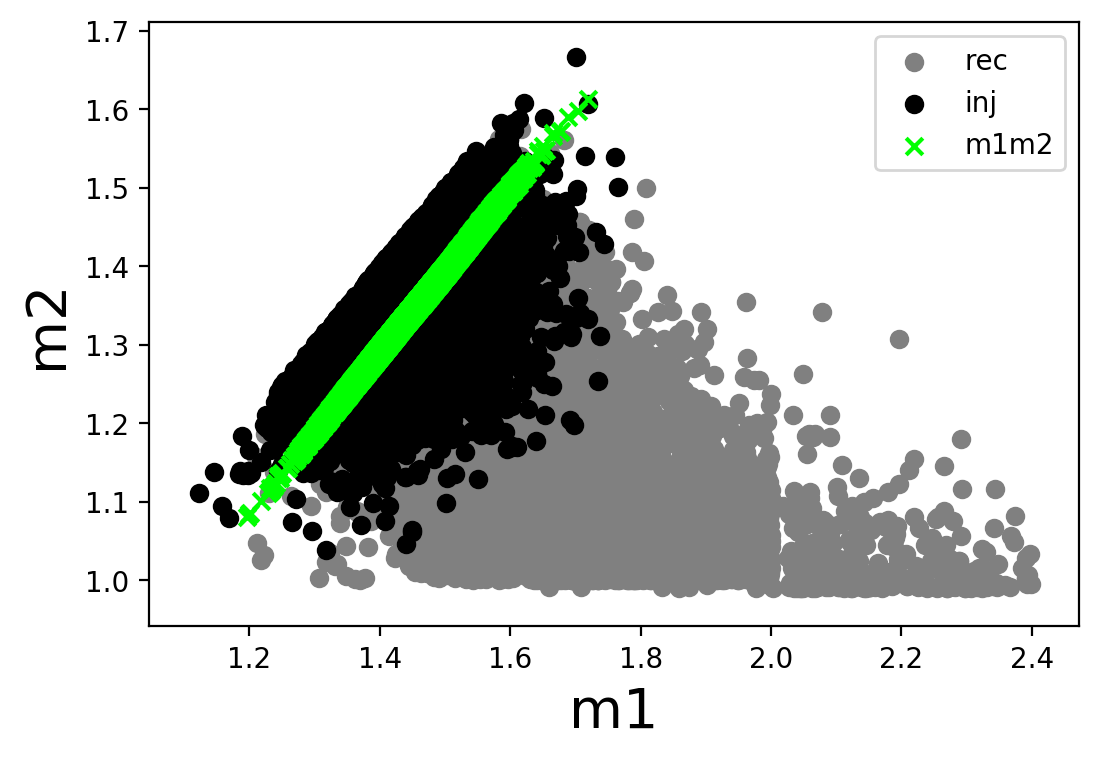
\includegraphics[width=0.28\textwidth]{./Figs/grey_m1m2.png}
  \includegraphics[width=0.28\textwidth]{./Figs/grey_m1Mc.png}
  \includegraphics[width=0.28\textwidth]{./Figs/grey_m1q.png} \\
  \rule[1ex]{14cm}{0.5pt}\\
  \includegraphics[width=0.28\textwidth]{./Figs/muMc_rainbow_m1m2.png}
  \includegraphics[width=0.28\textwidth]{./Figs/muMc_rainbow_m1Mc.png}
  \includegraphics[width=0.28\textwidth]{./Figs/muMc_rainbow_m1q.png} \\
  \includegraphics[width=0.28\textwidth]{./Figs/muMc_err_m1m2.png}
  \includegraphics[width=0.28\textwidth]{./Figs/muMc_err_Mc.png}
  \includegraphics[width=0.28\textwidth]{./Figs/muMc_err_q.png} \\
  \rule[1ex]{14cm}{0.5pt}\\
  \includegraphics[width=0.28\textwidth]{./Figs/p3Mc_rainbow_m1m2.png}
  \includegraphics[width=0.28\textwidth]{./Figs/p3Mc_rainbow_m1Mc.png}
  \includegraphics[width=0.28\textwidth]{./Figs/p3Mc_rainbow_m1q.png} \\
  \includegraphics[width=0.28\textwidth]{./Figs/p3Mc_err_m1m2.png}
  \includegraphics[width=0.28\textwidth]{./Figs/p3Mc_err_Mc.png}
  \includegraphics[width=0.28\textwidth]{./Figs/p3Mc_err_q.png} \\
  \rule[1ex]{14cm}{0.5pt}\\
  \includegraphics[width=0.28\textwidth]{./Figs/p3s_rainbow_m1m2.png}
  \includegraphics[width=0.28\textwidth]{./Figs/p3s_rainbow_m1Mc.png}
  \includegraphics[width=0.28\textwidth]{./Figs/p3s_rainbow_m1q.png} \\
  \includegraphics[width=0.28\textwidth]{./Figs/p3s_err_m1m2.png}
  \includegraphics[width=0.28\textwidth]{./Figs/p3s_err_Mc.png}
  \includegraphics[width=0.28\textwidth]{./Figs/p3s_err_q.png} \\
  \caption{\label{fig:epochs} Results for different epochs. Order:
  $(m_1, m_2)$, $(\mu, \Mc)$, $(p^3, \Mc)$, $(p^3, s)$, where
  $p=m_1 m_2$ and $s=m_1+m_2$. Layer (100,), $N_{\rm batch}=128$. 
  See Sec.~\ref{sec:epochs} for discussion. }
\end{figure*}
%
In this section we analyze the impact of the number of epochs used during the train. See the notebook \texttt{NN{\_}GSTLAL{\_}epochs.ipynb} for details.
The results using $N_{\rm batch}´ = 128$ and one hidden
layer with 100 neurons (502 trainable parameters) are shown in Fig.~\ref{fig:epochs}.
In the first row we show the usual plots for the standard regression $(m_1, m_2)$, 
nothing new except the very cool choice of colors for injected (black), recovered (grey),
and predicted (green). We train the NN for 50 epochs (with $(m_1, m_2)$
the number of epochs doesn't seem to matter a lot, 50 is well beyond the saturation). 
In the next three blocks we show the results of different regressions:
$(\mu, \Mc)$, $(p^3, \Mc)$, and $(p^3, s)$, where $p=m_1 m_2$ and $s=m_1+m_2$.
For each choice of features, we train the model for a different
number of epochs: 10, 25, 50, 100, 150, 200, 250, and 300.
The 'rainbow' plots are the usual plots of $m_2$, $\Mc$, and $q$ against $m_1$, 
but here each color is obtained training the NN for a different number of epochs;
the red point corresponds to 300 epochs. Below the 'rainbow' plots we
show the mean errors for $m_1$, $m_2$, $\Mc$, and $q$. The horizontal lines
mark the mean errors that correspond to the standard regression
on $(m_1, m_2)$ with 50 epochs. The regression with 
$(\mu, \Mc)$ does not seem to solve the $q$-problem, so it is ruled out\footnote{If we
care about $m_1$ and $m_2$!}.
$(p^3, \Mc)$ and $(p^3, s)$ are more promising, however in both cases 
the coverage seems to decrease with the number of epochs and the 
mean errors of $m_1$, $m_2$, and $q$ are bigger than in the $(m_1, m_2)$ regression. 
This could be an overfit-problem,
but on the other hand the mean error decrease with the number of epochs. 
In any case, the coverages of the parameter space are weird. 
Moreover, the final states are different from run to run (without changing anything
except the random initial state of the NN), so the methods do
not seem solid. However the restriction of the coverage and the decreasing 
of the mean errors with the number of epochs seems (more or less) a global trend.  

\subsection{Is the $q$-distribution in the injected data a problem?}
\label{sec:epochs_quniform}
%
\begin{figure}[]
  \center
  \includegraphics[width=0.47\textwidth]{./Figs/quniform_histo_inj.png}
  \rule[1ex]{7cm}{0.5pt}\\
  \includegraphics[width=0.47\textwidth]{./Figs/quniform_histo_rec.png}
  \caption{\label{fig:histo_quniform} Histogram for the $q$-uniform dataset.
  First row: injected, second row: recovered. }
\end{figure}
%
\begin{figure*}[]
  \center
  \includegraphics[width=0.28\textwidth]{./Figs/quniform_grey_m1m2.png}
  \includegraphics[width=0.28\textwidth]{./Figs/quniform_grey_m1Mc.png}
  \includegraphics[width=0.28\textwidth]{./Figs/quniform_grey_m1q.png} \\
  \rule[1ex]{14cm}{0.5pt}\\
  \includegraphics[width=0.28\textwidth]{./Figs/quniform_muMc_rainbow_m1m2.png}
  \includegraphics[width=0.28\textwidth]{./Figs/quniform_muMc_rainbow_m1Mc.png}
  \includegraphics[width=0.28\textwidth]{./Figs/quniform_muMc_rainbow_m1q.png} \\
  \includegraphics[width=0.28\textwidth]{./Figs/quniform_muMc_err_m1m2.png}
  \includegraphics[width=0.28\textwidth]{./Figs/quniform_muMc_err_Mc.png}
  \includegraphics[width=0.28\textwidth]{./Figs/quniform_muMc_err_q.png} \\
  \rule[1ex]{14cm}{0.5pt}\\
  \includegraphics[width=0.28\textwidth]{./Figs/quniform_p3Mc_rainbow_m1m2.png}
  \includegraphics[width=0.28\textwidth]{./Figs/quniform_p3Mc_rainbow_m1Mc.png}
  \includegraphics[width=0.28\textwidth]{./Figs/quniform_p3Mc_rainbow_m1q.png} \\
  \includegraphics[width=0.28\textwidth]{./Figs/quniform_p3Mc_err_m1m2.png}
  \includegraphics[width=0.28\textwidth]{./Figs/quniform_p3Mc_err_Mc.png}
  \includegraphics[width=0.28\textwidth]{./Figs/quniform_p3Mc_err_q.png} \\
  \rule[1ex]{14cm}{0.5pt}\\
  \includegraphics[width=0.28\textwidth]{./Figs/quniform_p3s_rainbow_m1m2.png}
  \includegraphics[width=0.28\textwidth]{./Figs/quniform_p3s_rainbow_m1Mc.png}
  \includegraphics[width=0.28\textwidth]{./Figs/quniform_p3s_rainbow_m1q.png} \\
  \includegraphics[width=0.28\textwidth]{./Figs/quniform_p3s_err_m1m2.png}
  \includegraphics[width=0.28\textwidth]{./Figs/quniform_p3s_err_Mc.png}
  \includegraphics[width=0.28\textwidth]{./Figs/quniform_p3s_err_q.png} \\
  \caption{\label{fig:epochs_quniform} Results for different epochs on q-uniform dataset. Order:
  $(m_1, m_2)$, $(\mu, \Mc)$, $(p^3, \Mc)$, $(p^3, s)$, where
  $p=m_1 m_2$ and $s=m_1+m_2$. Layer (100,), $N_{\rm batch}=128$. 
  See Sec.~\ref{sec:epochs} and Sec.~\ref{sec:epochs_quniform} for discussion. }
\end{figure*}
%
In Sec.~\ref{sec:GstLALanalysis} we saw that the distribution of $q$ in
the injected data is not uniform. Is this a problem?
Short answer: not much. 
Long answer: we created a new dataset with uniform q-sampling in the injected data, 
the resulting mass distrubtions are shown in Fig.~\ref{fig:histo_quniform}.
Then using this dataset we run again the test on the epochs, obtaining 
Fig.~\ref{fig:epochs_quniform}. Now the mean errors are closer to the ones
obtained with the standard regression $(m_1, m_2)$, but be aware that
the latter are bigger than with the full dataset (not uniform in $q$).
In any case, the coverage of the parameter space is still an issue. 


%==========================================================
\section{Things to discuss}
%==========================================================
\begin{itemize}
\item The regression with NNs does not work properly on the GstLAL BNS dataset. SOLVED: this is a mix of  data not sampled uniformly and bad design of the NN (Simone: is this really solved?).

\item Improve the loss function. We can add information even if it is not a parameter to do regression to. See section \ref{sec:loss_new}. Simone can you implement this?

\item Does GPR face the same issues? Try with $m1,m2$, and the approach with parameters $p$ and $s$. If it performs better than the NN, then it is a matter of the loss function for the NN now. 

\item Improve fake-fake data? Not at the moment.

\item Since we are starting to use more complex NNs (at least for \texttt{NewRealistic} 
datasets, i.e. \texttt{v0c0} and \texttt{v1c0}), should we try to use some dropout?
[not a first order priority in any case]
\end{itemize}
%==========================================================
\bibliography{refs,local}
%==========================================================

\end{document}